\documentclass{beamer}
%\usepackage{polski}
\usepackage[utf8]{inputenc}
\usepackage{graphicx}
\usepackage{ragged2e}


\usepackage{hyperref}
\usepackage{amsmath}
\usepackage{amsfonts}
\usepackage{amsthm}
\usepackage{amssymb}
\usepackage{amstext}
\usepackage{graphicx}
\usepackage{indentfirst}
\usepackage{blkarray}
\usepackage{url}
\usepackage{multirow}
\usepackage{fancyhdr}
\usepackage{listings}
\usepackage{setspace}
\usepackage{subfigure}
\usepackage{appendixnumberbeamer}
\usepackage{lipsum}
\usepackage{colortbl}
\usepackage{hyperref}
\usepackage{xcolor}
%\usepackage{ctable}

\newcommand{\backupbegin}{
   \newcounter{finalframe}
   \setcounter{finalframe}{\value{framenumber}}
}
\newcommand{\backupend}{
   \setcounter{framenumber}{\value{finalframe}}
}

\useoutertheme{infolines}

\usetheme{Madrid}
\usecolortheme{default}

\title[cfluxim cosmic ray simulation tool]{\texttt{cfluxim}\\cosmic ray simulation tool}
\subtitle{}
\author[K. Wójcik]{Kamil Wójcik}
\institute[University of Silesia]{University of Silesia}
\date{2020}

\begin{document}
%%%%%%%%%%%%%%%%%%%%%%%%%%%%%%%%%%%%%%%%%%%%%%%%%%%%%%%%%%%%%%%%%%
\begin{frame}
	\vfill
	\titlepage
	\vfill
	\usebeamerfont{institute}
	\center{\url{kamil.wojcik@us.edu.pl}}
\end{frame}
%%%%%%%%%%%%%%%%%%%%%%%%%%%%%%%%%%%%%%%%%%%%%%%%%%%%%%%%%%%%%%%%%%%%%%%%%%%%%%%%%%


	\begin{frame}
		\frametitle{Contents}
		\tableofcontents
	\end{frame}


\section{General information}

\begin{frame}
\vfill
\centering
\Huge{General information}

\vfill
\end{frame}



\begin{frame}{About cfluxim}

The \texttt{cfluxim} project was created to make a simple geometrical simulation of cosmic muons passing through some modules of the MPD detector (\textcolor{blue}{\href{https://nica.jinr.ru/projects/mpd.php}{NICA MPD website}}).

\begin{itemize}
\item Cosmic muons are generated inside the given cubic volume.
\item $\Phi(\theta)$ and momentum distribution of the simulated flux fits the the experimental data with good accuracy.
\item For every generated particle, it is checked if it hits the defined detector modules, and the hit position is saved.
\item Any energy cutoff can be applied.
\end{itemize}

\end{frame}

\begin{frame}{General notes}
\begin{itemize}
\item \texttt{cfluxim} uses \textcolor{blue}{\href{https://root.cern/}{CERN's ROOT}} libraries.
\item \texttt{cfluxim} consists of 3 tools: \texttt{CuboidGenerator}, \texttt{FluxAnalyzer} and \texttt{TrackAnalyzer}.
\item Only muons at ground level are implemented, however, implementation of other cosmic ray components is possible.
\item \texttt{FluxAnalyzer} generates momentum distribution and $\Phi(\theta)$ normalized histogram, so it can be compared wirh the experimental data as a simple quality check.
\item \texttt{TrackAnalyzer} does the simple geometrical analysis of the tracks, regarding the defined detector geometry. It does not run the full physical analysis as \textcolor{blue}{\href{https://geant4.web.cern.ch/}{Geant4}} does.
\item Generated cosmic muons can be, however, put into the Geant4 simulation.
\end{itemize}
\end{frame}

\begin{frame}{Project scheme}
\begin{figure}
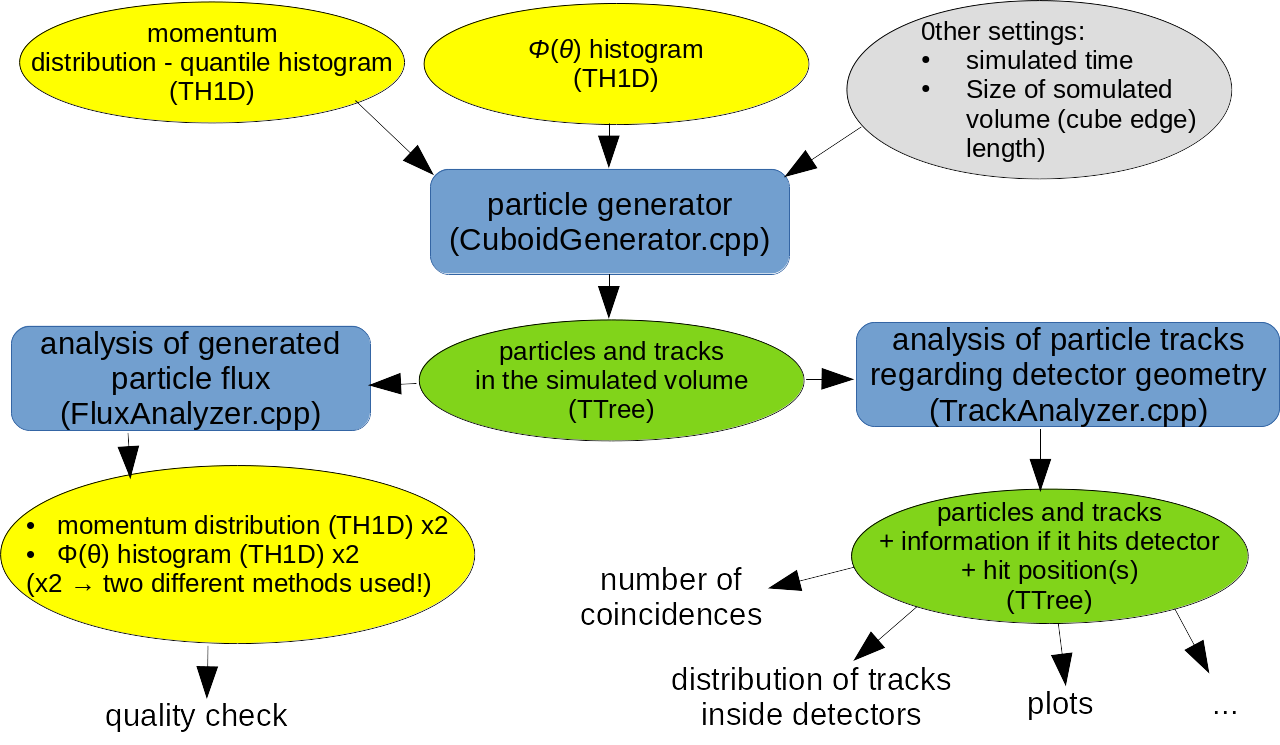
\includegraphics[width=\textwidth]{images/sim_scheme.png}
\end{figure}
s\end{frame}


\section{Cosmic ray flux -- definition}

\begin{frame}
\vfill
\centering
\Huge{Basic definitions}

\vfill
\end{frame}

\begin{frame}{Solid angle}
\begin{figure}
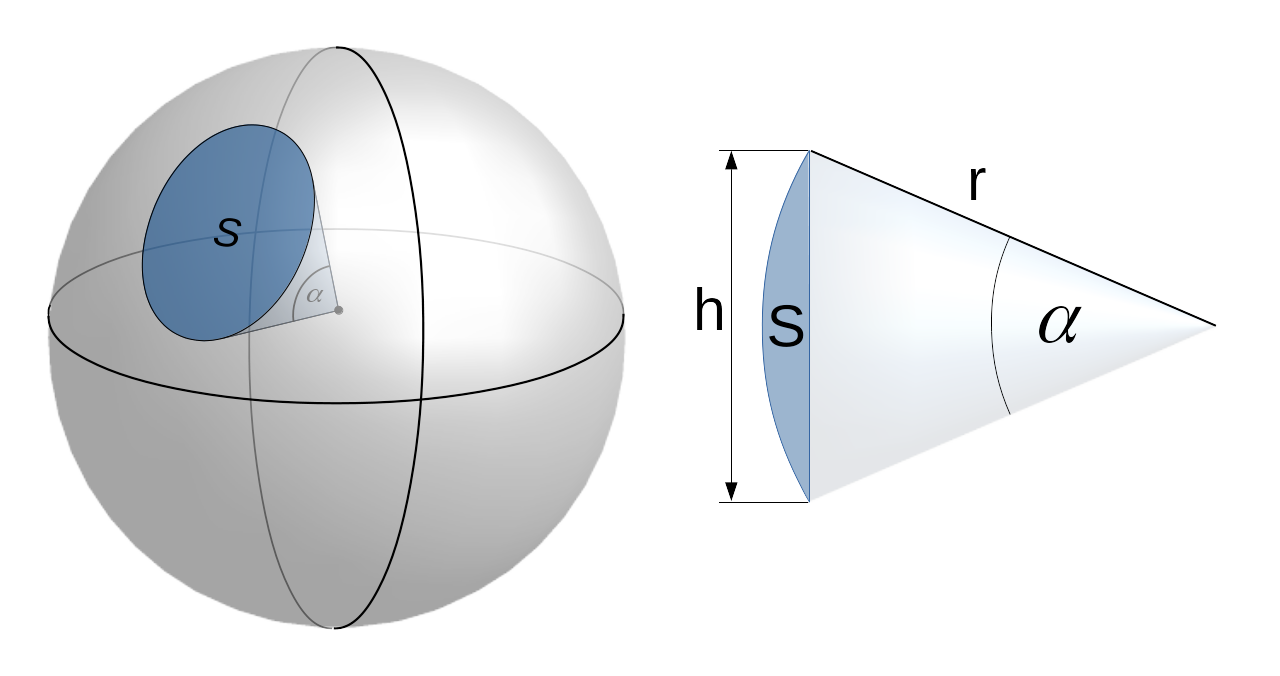
\includegraphics[width=0.9\textwidth]{images/solid_angle.png}%
\end{figure}
\centering
area: ~~$S= 2 \pi r h = 2 \pi r^2 (1-cos \alpha)$\\
solid angle: ~~$\Omega= \frac{S}{r^2}=2 \pi (1-cos \alpha) ~ \text{[sr]}$
\end{frame}

\begin{frame}{Cosmic ray flux}
\centering
\emph{ Cosmic ray flux~~=~~ number of particles that come from unit solid angle, passing through unit area, per unit of time}
~\\~\\

\begin{figure}
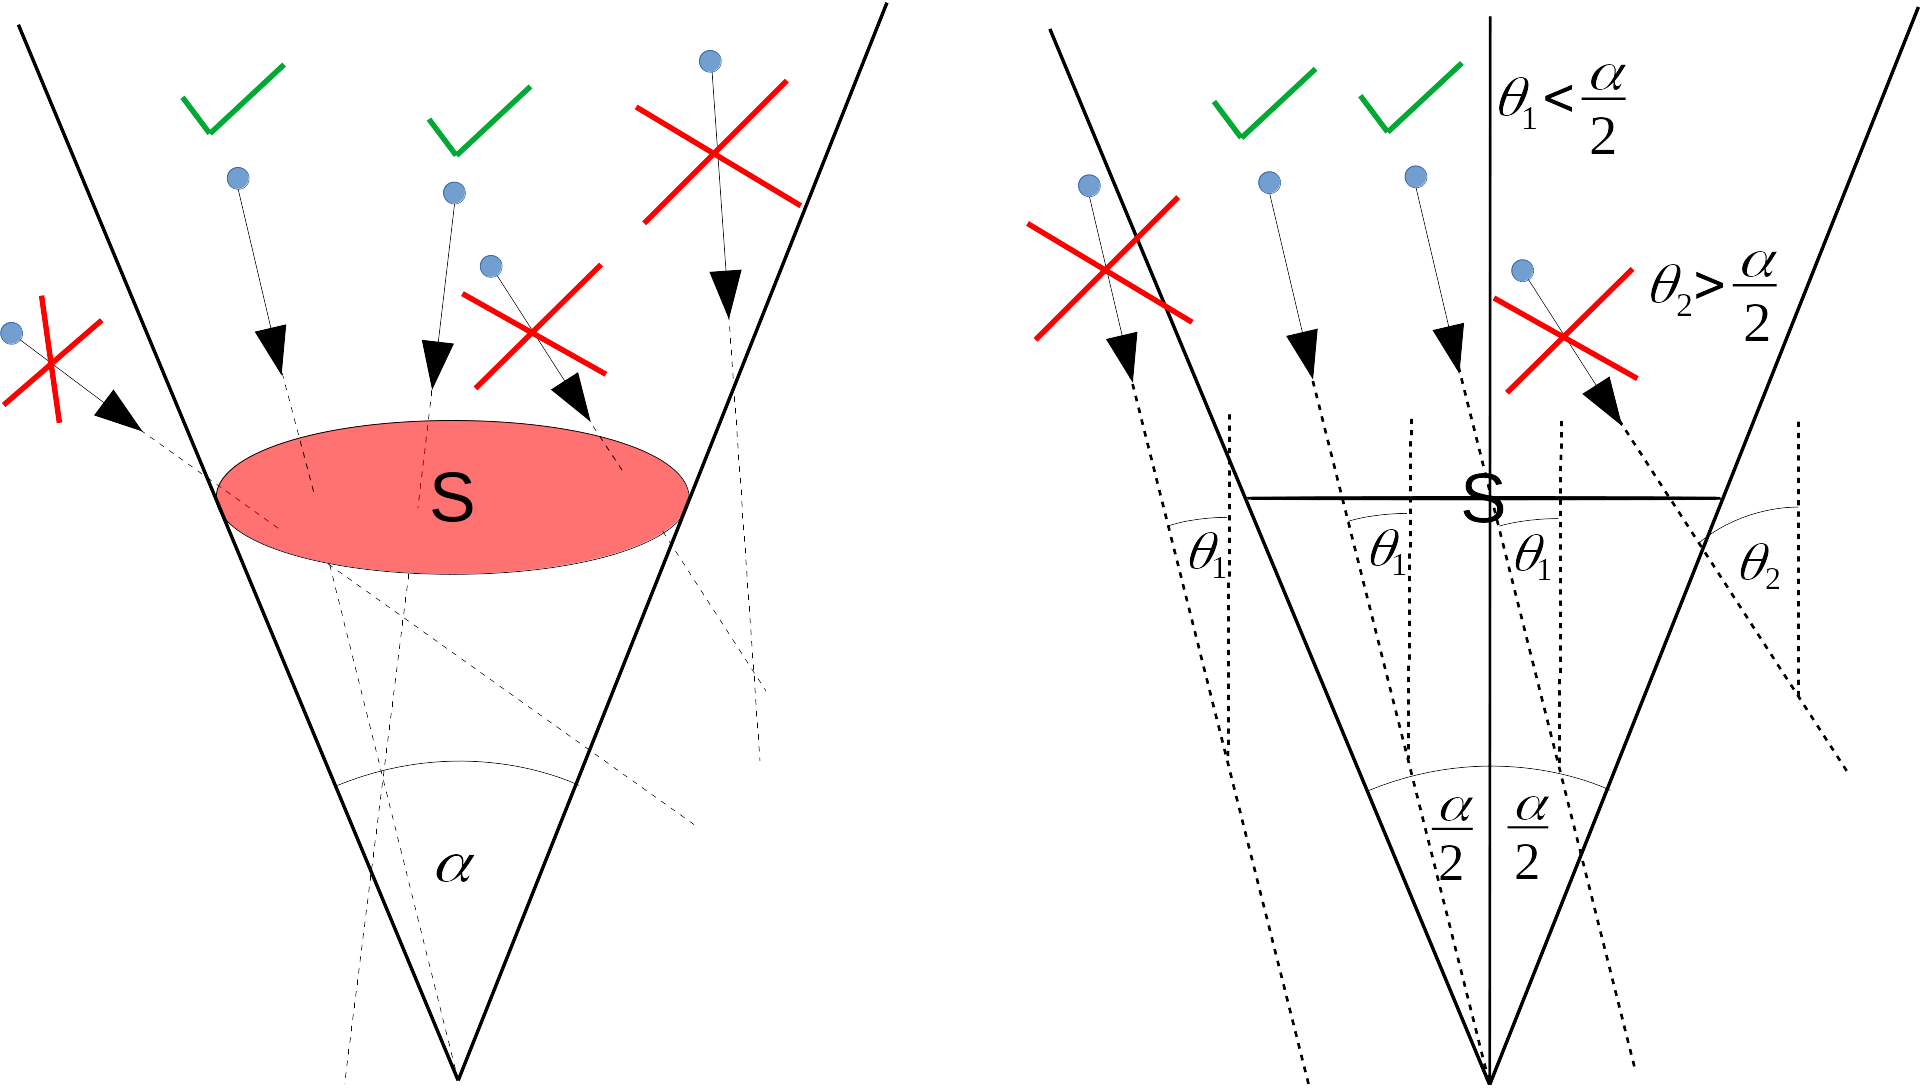
\includegraphics[width=0.62\textwidth]{images/steradianDef.png}~
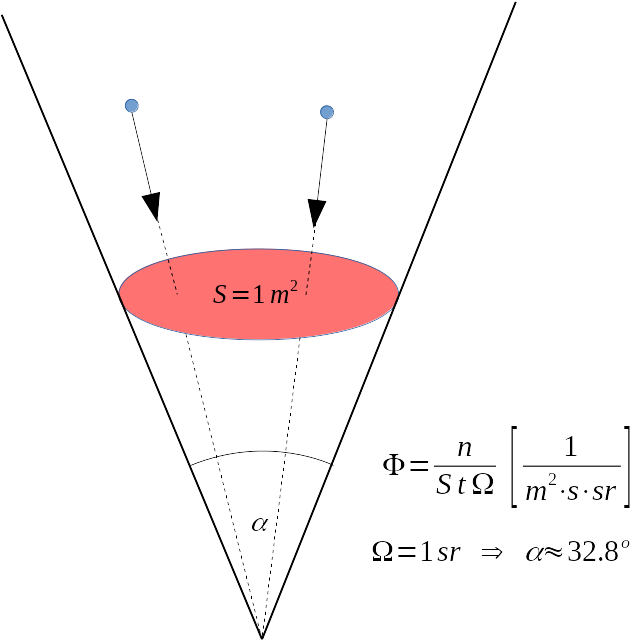
\includegraphics[width=0.36\textwidth]{images/steradian_normalization.png}\\
particles coming from a given solid angle~~~~~~~~standard~normalization~~~~\\
passing through area S~~~~~~~~~~~~~~~~~~~~~~~~~~~~~~~~~~~~~
\end{figure}
\end{frame}

\begin{frame}{Cosmic ray flux}

\begin{figure}
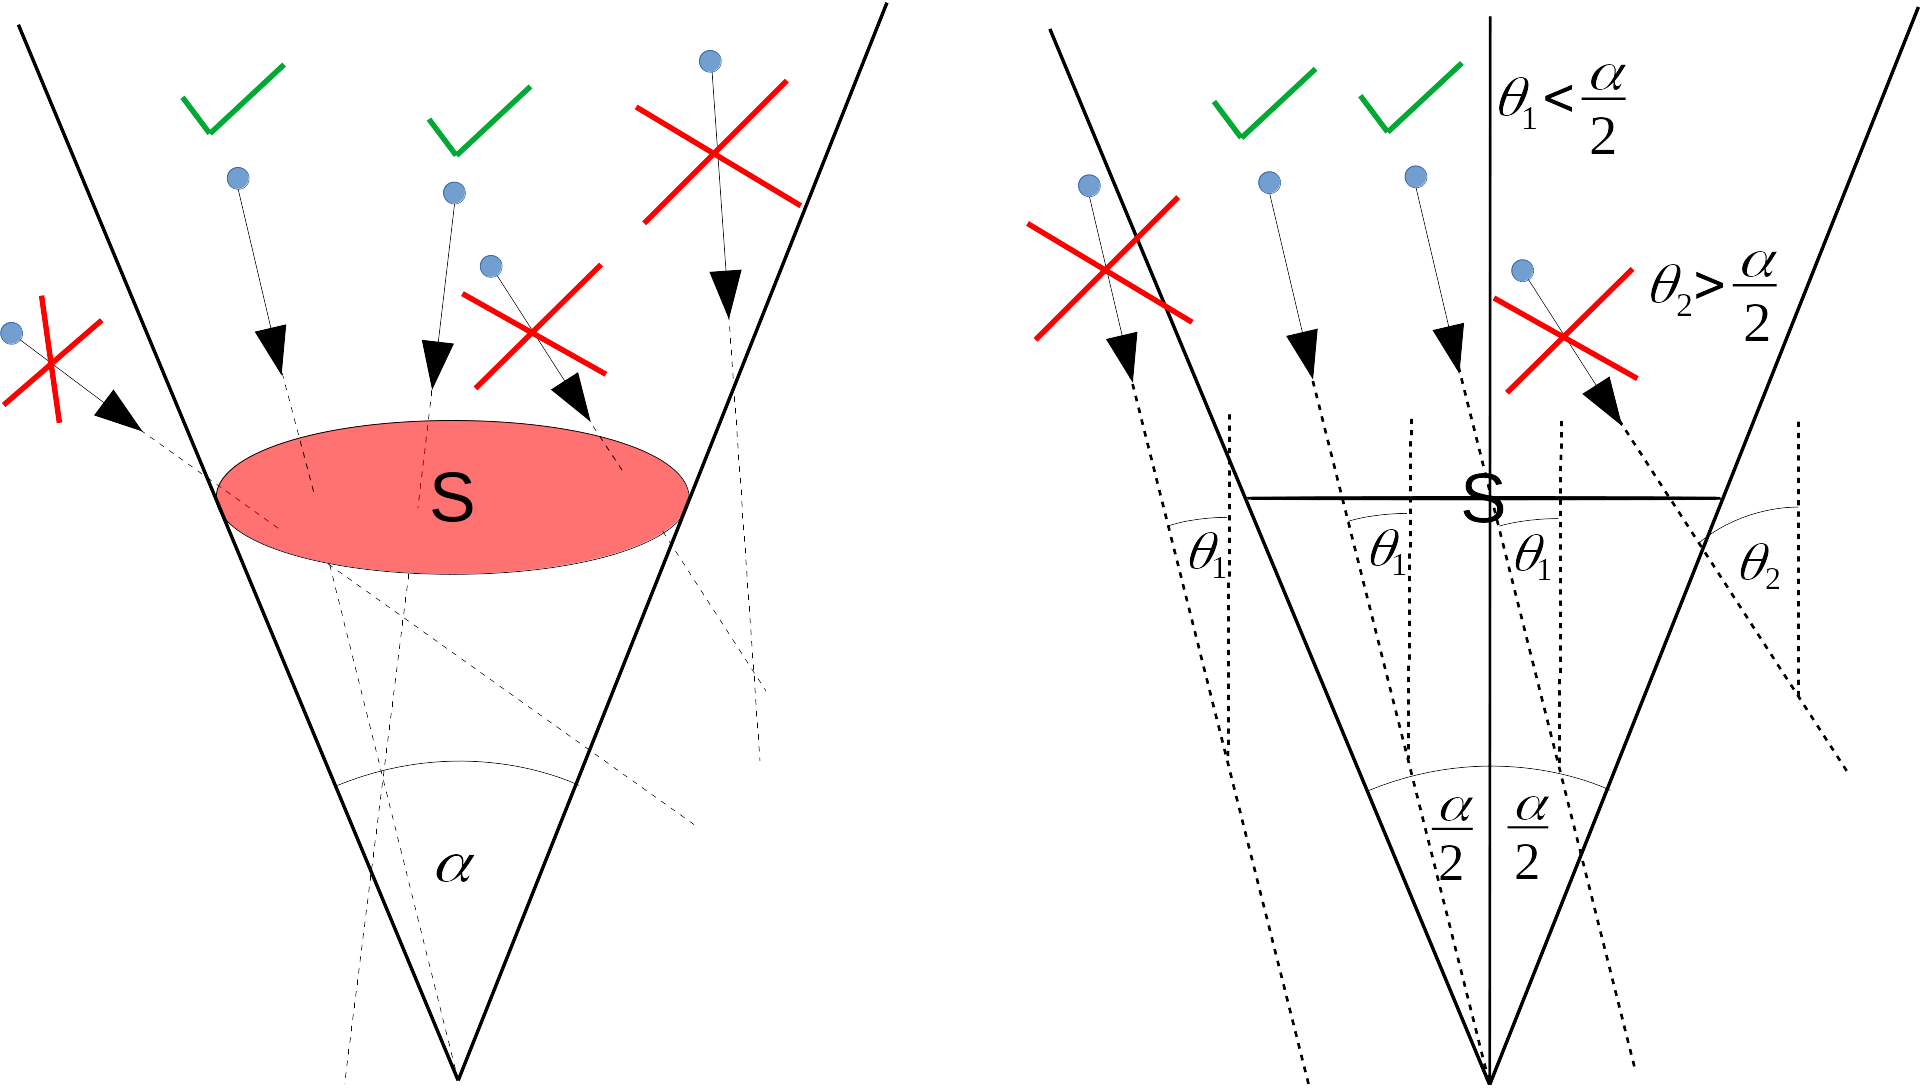
\includegraphics[width=0.8\textwidth]{images/steradianDef.png}~
\end{figure}
Solid angle limits the $direction$ of incoming particle momentum, but not the position on the `probing area' $S$. To count a particle as coming from the given solid angle, momentum angular limitations must be fulfilled and the particle must hit the probing area.
\end{frame}

\begin{frame}{Cosmic ray flux dependant on zenith angle}
\begin{figure}
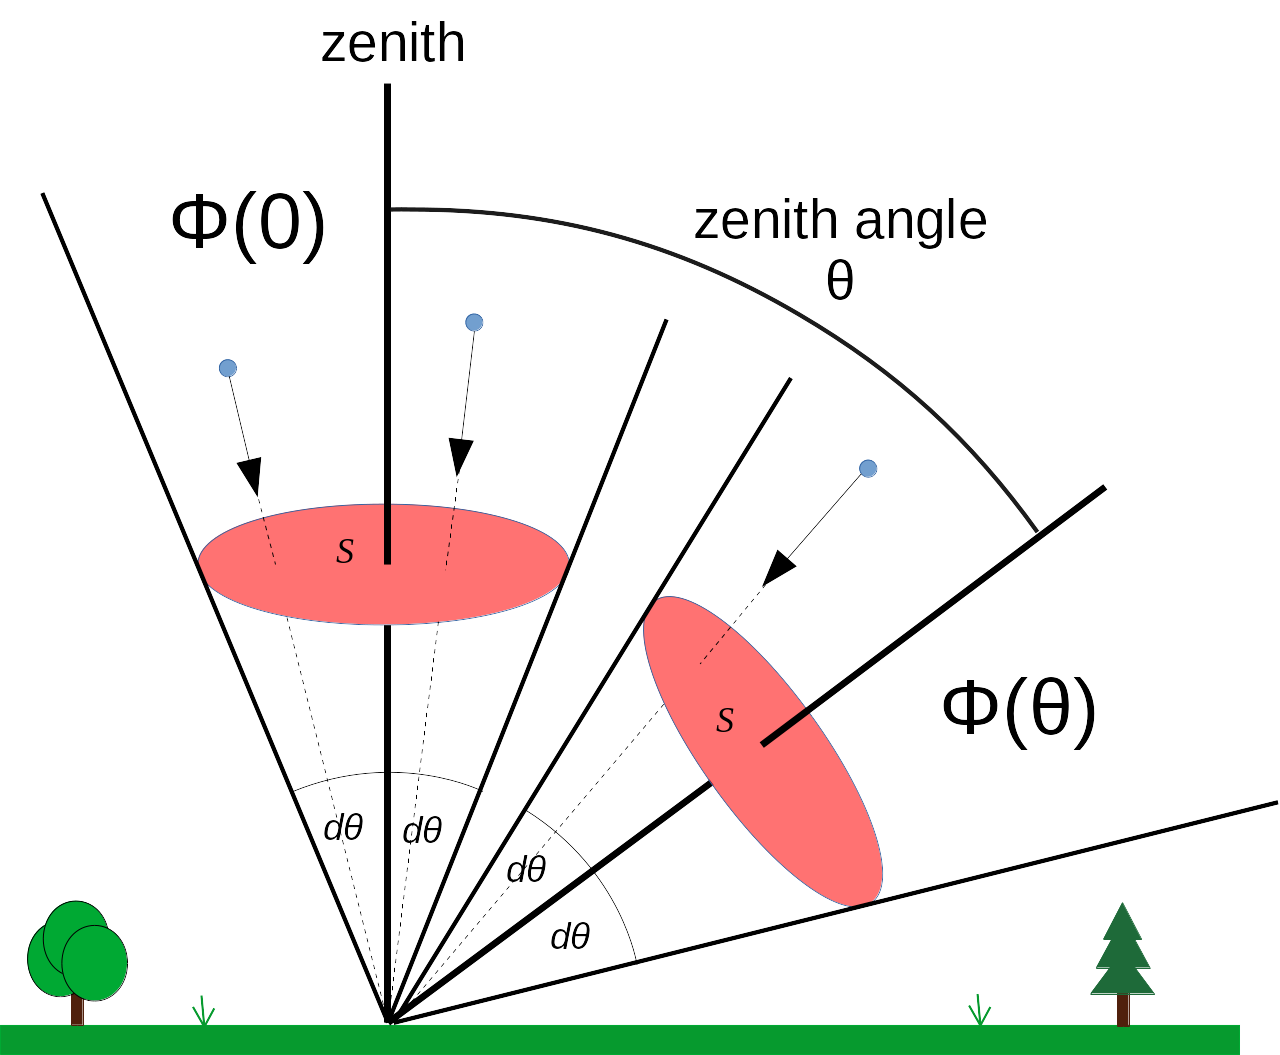
\includegraphics[width=0.7\textwidth]{images/fluxZenithAngleDef.png}%
\end{figure}
\end{frame}

\begin{frame}{Cosmic ray flux dependant on zenith angle\\-- full azimuth angle case}
\begin{figure}
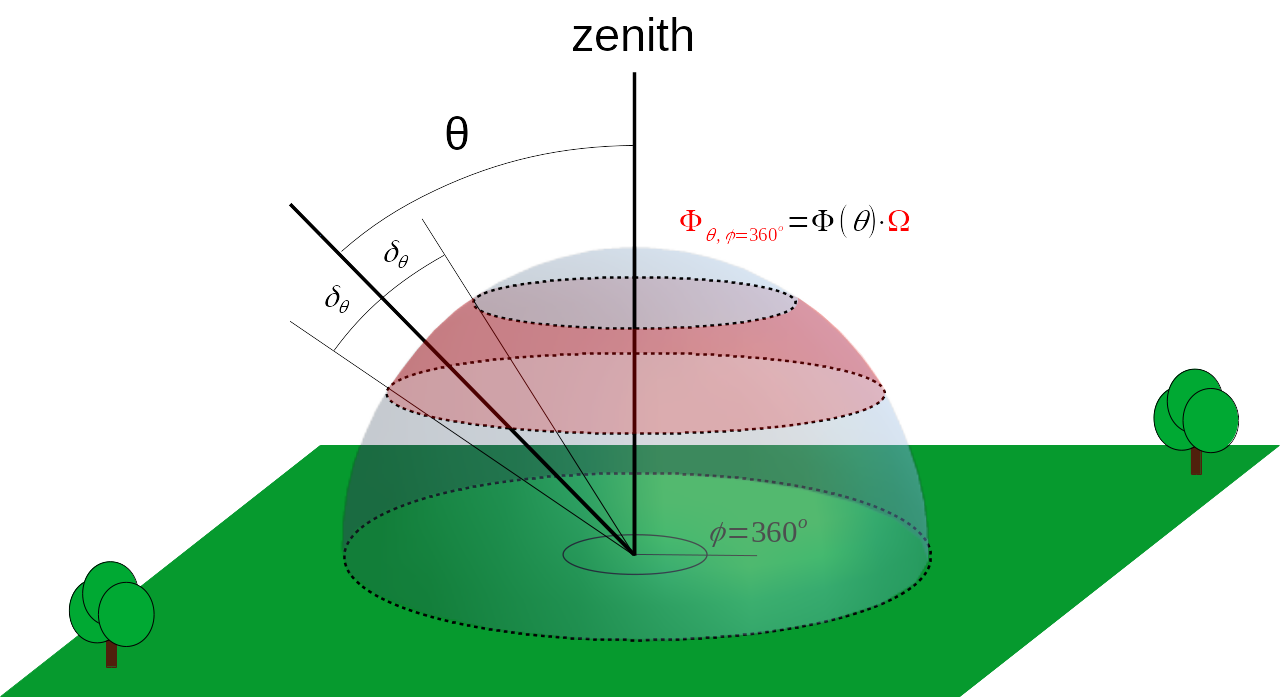
\includegraphics[width=0.95\textwidth]{images/fluxZenith.png}%
\end{figure}
\[
\textcolor{red}{\Omega} = 2\pi (cos (\theta - \delta_\theta) - cos(\theta + \delta_\theta))
\]


\end{frame}

\section{Simulation design}

\begin{frame}
\vfill
\centering
\Huge{Simulation design}

\vfill
\end{frame}

\subsection{CuboidGenerator}

\begin{frame}{\texttt{CuboidGenerator}}
\begin{figure}
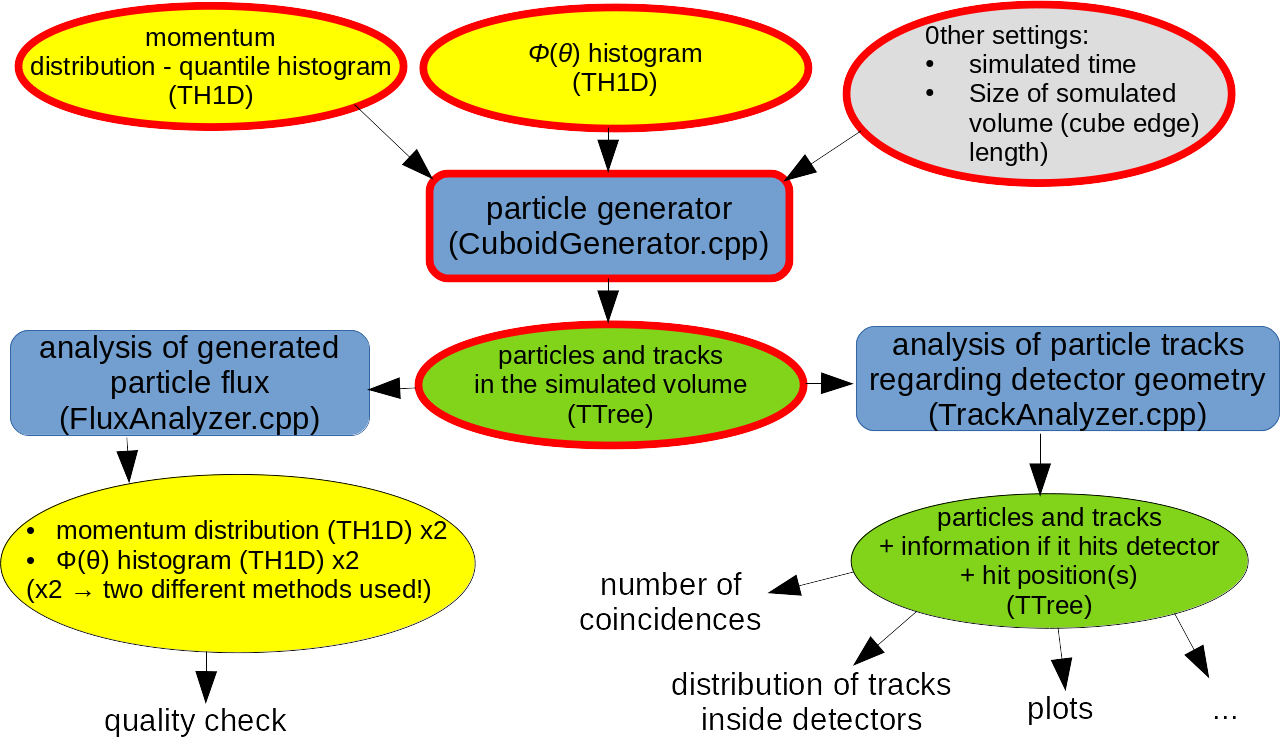
\includegraphics[width=0.9\textwidth]{images/sim_scheme_cuboid.png}%
\end{figure}
\end{frame}

\begin{frame}{\texttt{CuboidGenerator} -- the idea}

The idea: generation of particles and its momenta, coming from half-sphere ($\Omega=2\pi$), that would pass through a cubic volume.
\begin{figure}
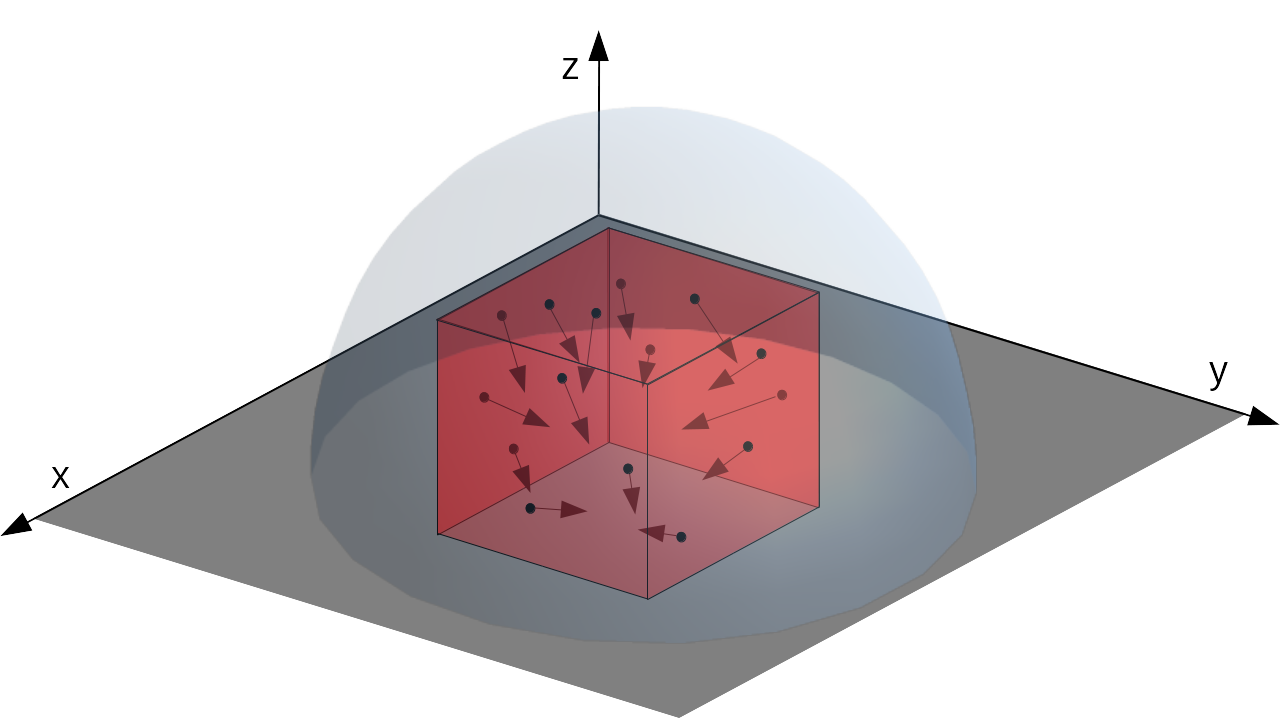
\includegraphics[width=0.5\textwidth]{images/cuboidIdea.png}
\end{figure}
Particle's `initial' position on the cube wall and its momentum vector define the track inside the cube!

Key problems:
\begin{itemize}
\item $\Phi(\theta)$ of generated particles must reproduct the experimental data with sufficient accuracy.
\item Same for momentum distribution.
\end{itemize}
\end{frame}

\begin{frame}{Horizontal area problem}

\begin{enumerate}
\item $2\pi$ solid angle is divided into small $\Omega_i$ solid angles
\item for each $\Omega_i$: the number of incoming particles from this $\Omega_i$ in simulated time $t_{sim}$ is calculated -- $N_i$  
\end{enumerate}

\begin{figure}
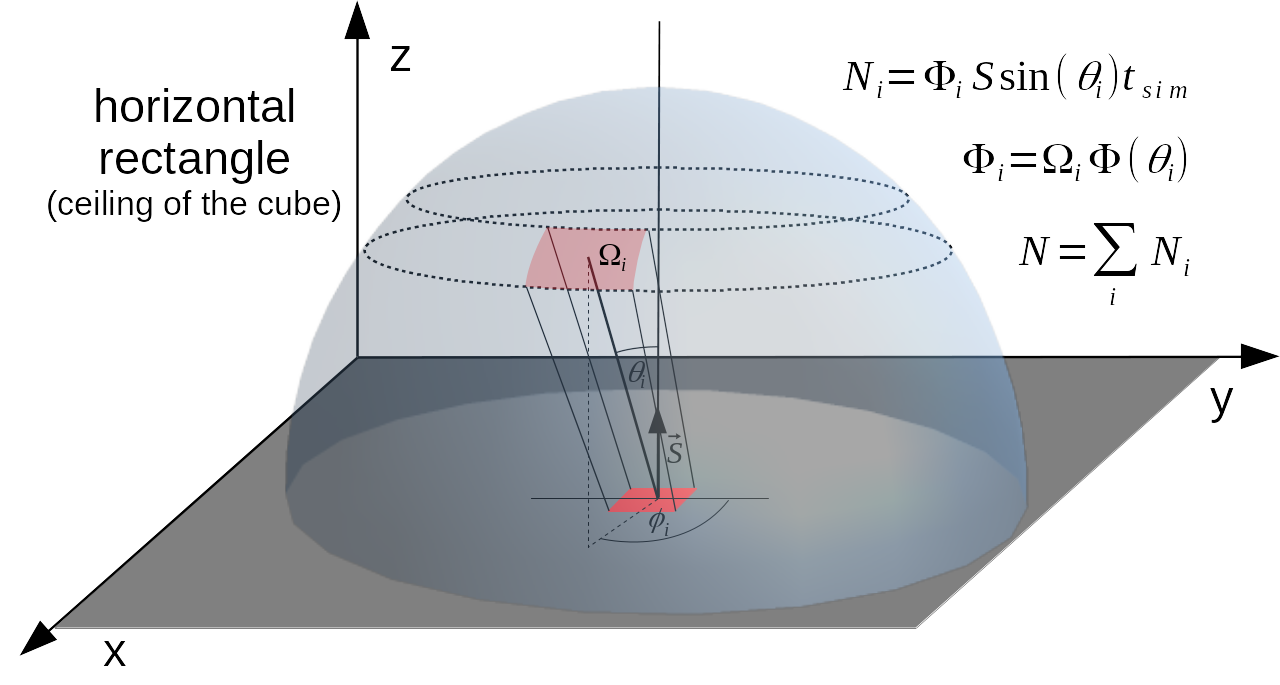
\includegraphics[width=\textwidth]{images/hor.png}
\end{figure}
\end{frame}


\begin{frame}{Horizontal area problem}

Number of incoming particles from $\Omega_i$ per second can be mapped, regarding $\theta_i$ and $\phi_i$:
\[
Npps_i =  \Omega_i \Phi(\theta_i) S sin(\theta_i)
\]
\begin{figure}
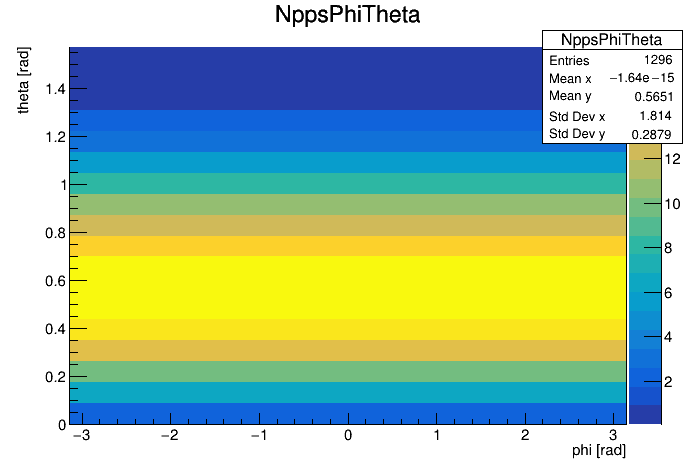
\includegraphics[width=0.6\textwidth]{images/CeilingFluxMap.png}
\end{figure}
The cube ceiling is horizontal $\Rightarrow$ flux depends only on $\theta$
\end{frame}

\begin{frame}{Vertical area problem}

\begin{enumerate}
\item $\Omega_i$ and $N_i$ -- same as for horizontal area
\item Only particles that come from one side of the wall are generated $\Rightarrow$ $\phi_i$ range is limited!
\item $N_i$ depends on both $\theta_i$ and $\phi_i$
\end{enumerate}

\begin{figure}
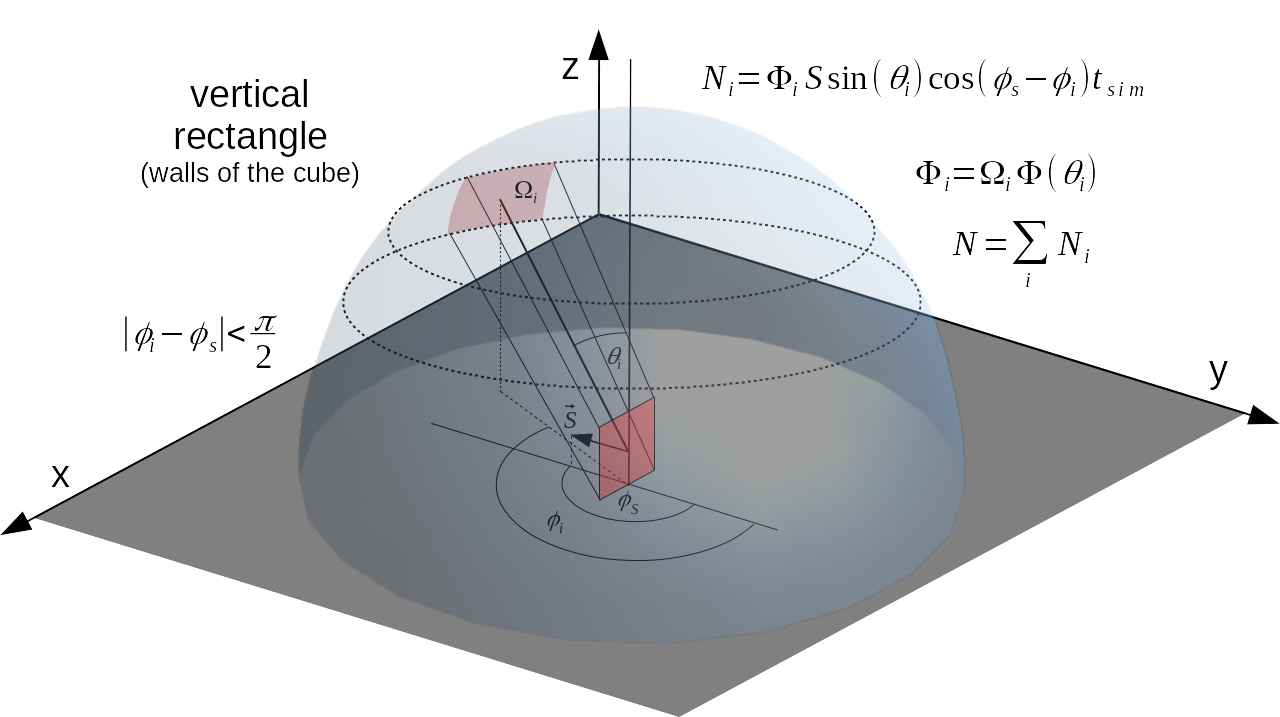
\includegraphics[width=0.8\textwidth]{images/ver.png}
\end{figure}
\end{frame}

\begin{frame}{Vertical area peoblem}
$Npps_i$ formula for vertical walls of the cube:
\[
Npps_i = \Omega_i \Phi(\theta_i) S sin(\theta_i) cos (\phi_s - \phi_i)
\]
\begin{figure}
~wall 1~~~~~~~~~~~~~~~~~~~~~~ wall 2\\
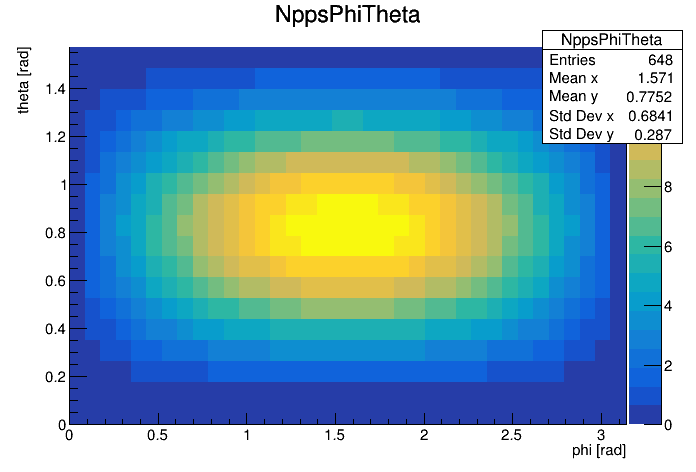
\includegraphics[width=0.32\textwidth]{images/Wall1FluxMap.png}%
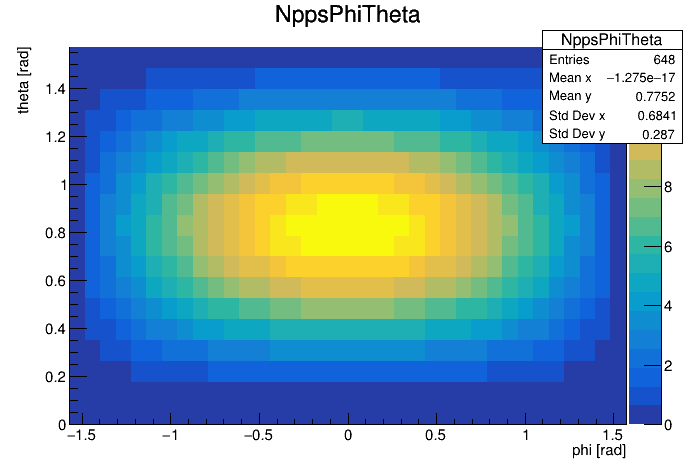
\includegraphics[width=0.32\textwidth]{images/Wall2FluxMap.png}\\
~wall 3~~~~~~~~~~~~~~~~~~~~~~ wall 4\\
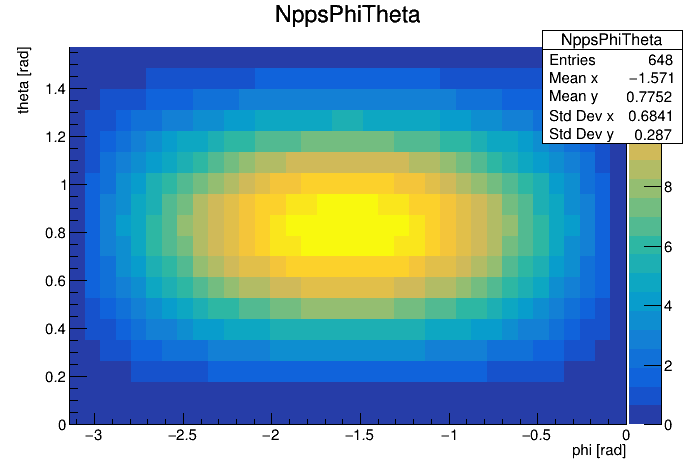
\includegraphics[width=0.32\textwidth]{images/Wall3FluxMap.png}%
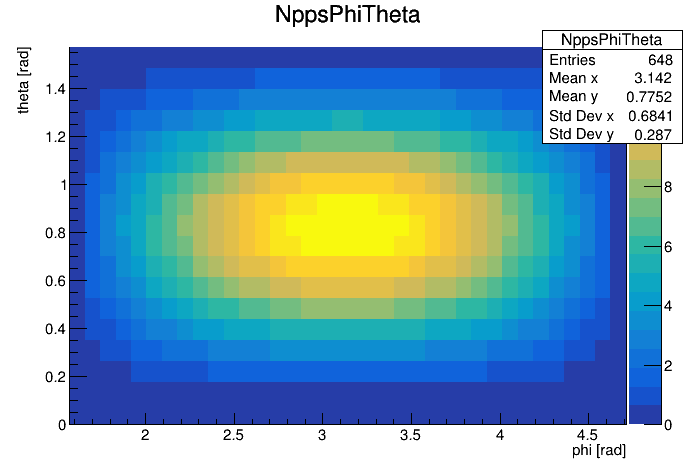
\includegraphics[width=0.32\textwidth]{images/Wall4FluxMap.png}\\
\end{figure}
\end{frame}

\begin{frame}{How momentum is generated}
These two histograms made from experimental data are necessary for momentum generation
\begin{figure}
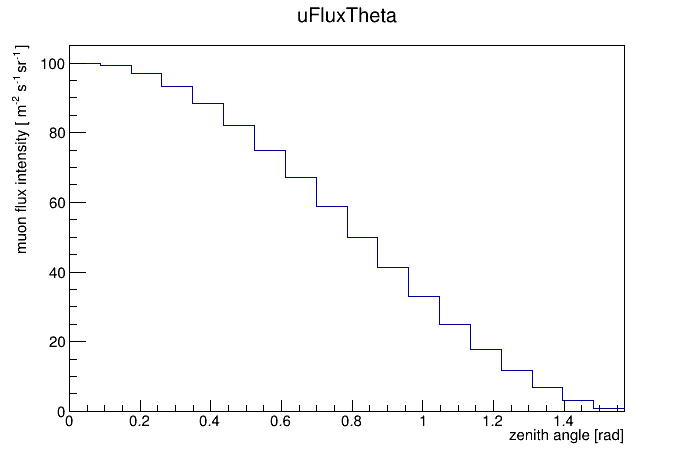
\includegraphics[width=0.52\textwidth]{images/uFluxTheta.png}%
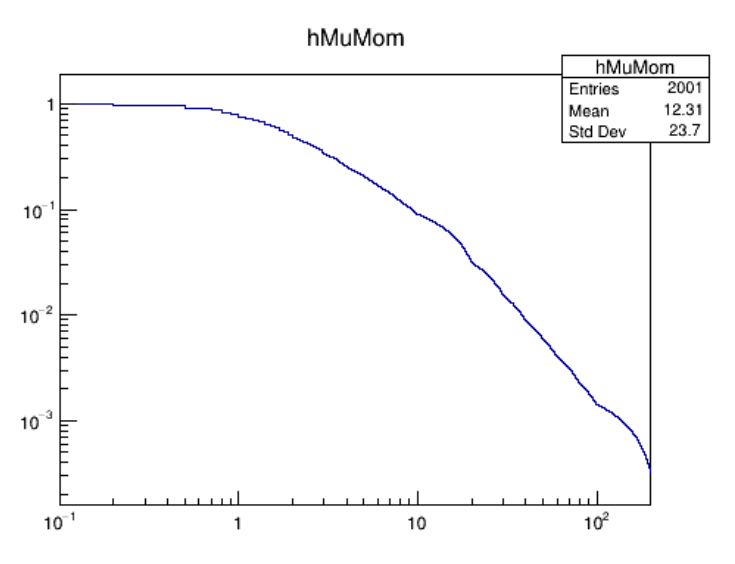
\includegraphics[width=0.46\textwidth]{images/hmomfull.png}
\end{figure}
\end{frame}

\begin{frame}{$\Phi(\theta)$ -- input histogram}
On the left: measured vertical muon flux at the sea level (log scale), fitted with `cosine function': $\Phi(\theta) = cos^2(\theta)$. Data source: \textcolor{blue}{\href{https://arxiv.org/pdf/1606.06907.pdf}{https://arxiv.org/pdf/1606.06907.pdf}}
\begin{figure}
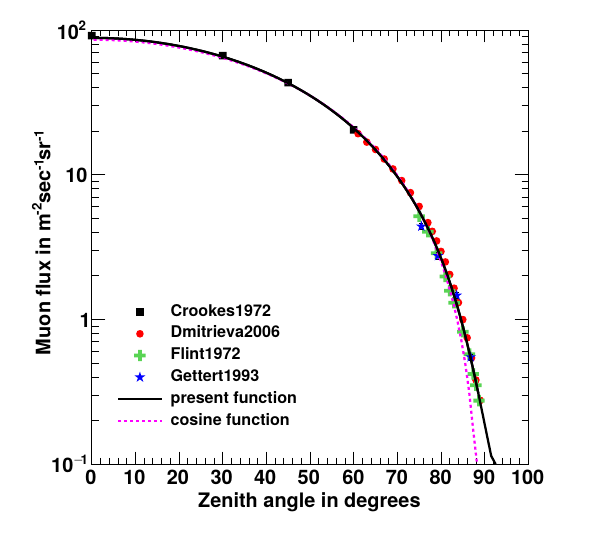
\includegraphics[width=0.41\textwidth]{images/cosine_experiment.png}%
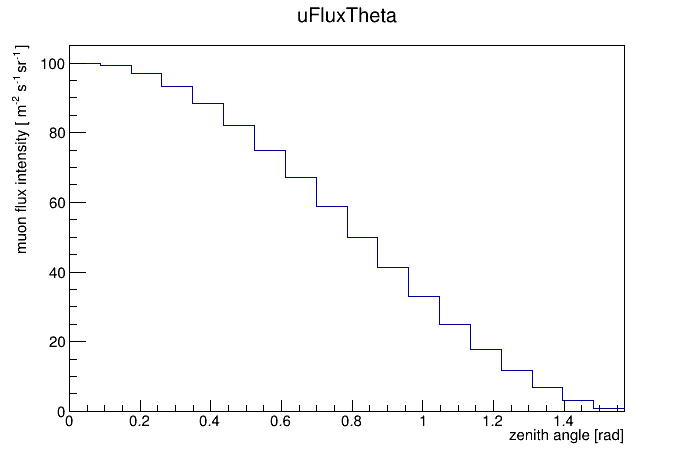
\includegraphics[width=0.58\textwidth]{images/uFluxTheta.png}
\end{figure}
On the right: the input hostogram of $\Phi(\theta)$ (linear scale). Since $cos^2(\theta)$ fits the data precisely enough, the histogram is just filled with $cos^2(\theta)$ distribution.
\end{frame}

\begin{frame}{$\Phi(\theta)$ and flux mapping  $\rightarrow ~ p_\theta$ and $p_\phi$}
1. Momentum coordinates $p_\theta$ and $p_\phi$ are limited by the solid angle $\Omega_i$:
\begin{figure}
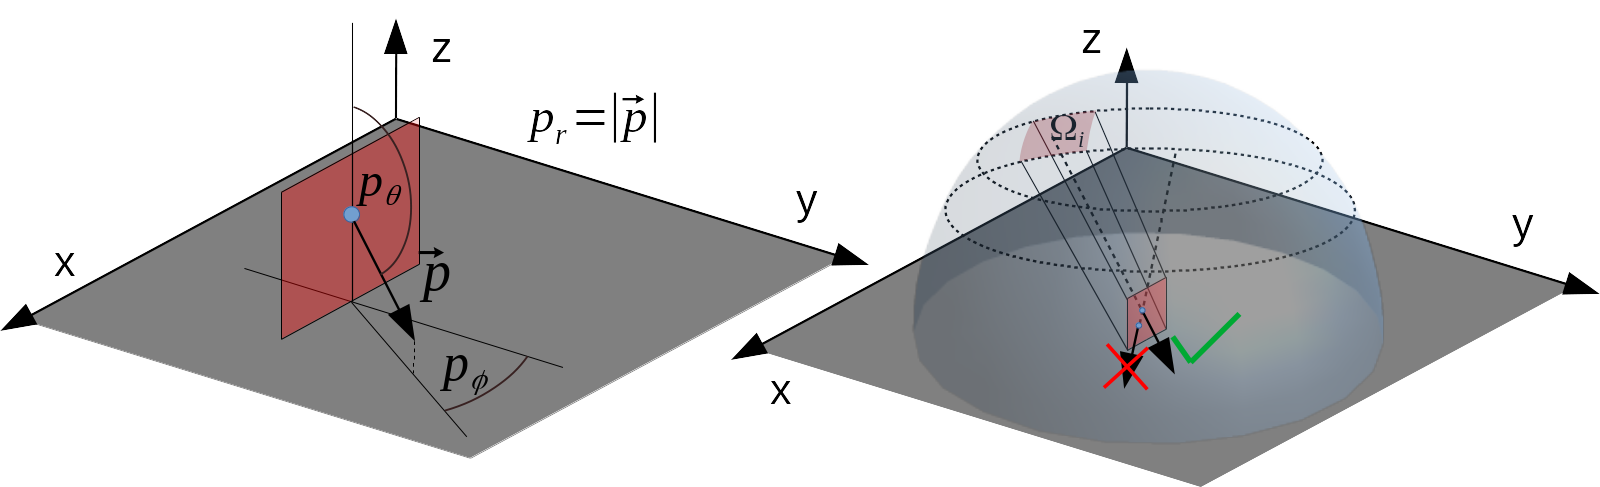
\includegraphics[width=1.02\textwidth]{images/p_spherical.png}%
\end{figure}
\end{frame}

\begin{frame}{$\Phi(\theta)$ and flux mapping  $\rightarrow ~ p_\theta$ and $p_\phi$}
2. Flux is mapped into $\theta$--$\phi$ space regarding $\Phi(\theta)$ histogram:
\begin{figure}
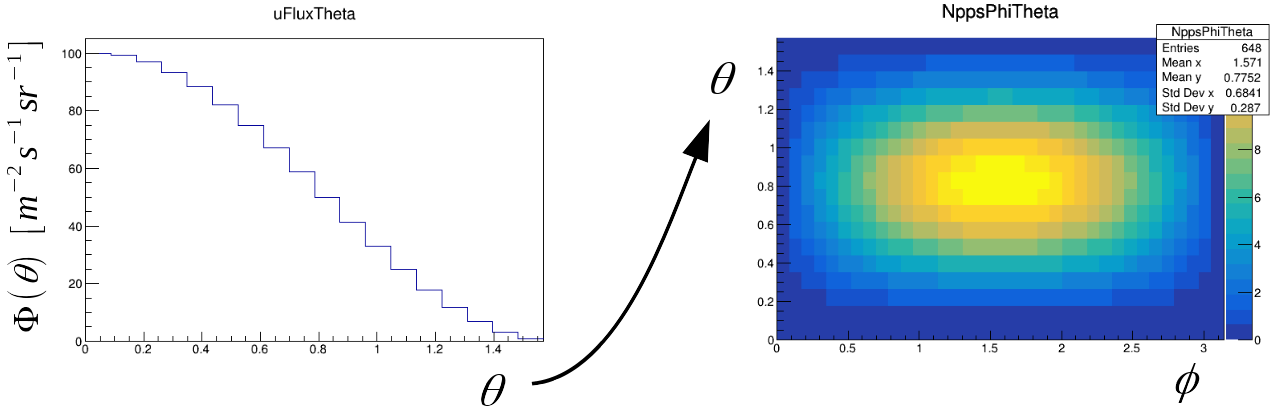
\includegraphics[width=0.8\textwidth]{images/Phi_theta_fluxmap.png}%
\end{figure}
\[
Npps_i \propto \Phi(\theta_i)
\]
3. $\Omega_i$ corresponds with the intervals: $[\theta_i,~\Delta_\theta)$ and $[\phi_i,~\Delta_\phi)$. Within the intervals,
$p_\theta$ and $p_\phi$ is drawn from uniform distrubution. \\~\\

4. \textbf{Generation of $N_i \propto Npps_i$ particles from each $\Omega_i$ solid angle guarantees that the given $\Phi(\theta)$  is reconstructed by the generated particles.} The accuracy of this reconstruction is sufficient if $\Delta \theta$ is small enough.
\end{frame}

\begin{frame}{$p_r$ distribution}
On the left: measured vertical integral spectra of muons. Data source: \textcolor{blue}{\href{http://crd.yerphi.am/Muons}{http://crd.yerphi.am/Muons}}
\begin{figure}
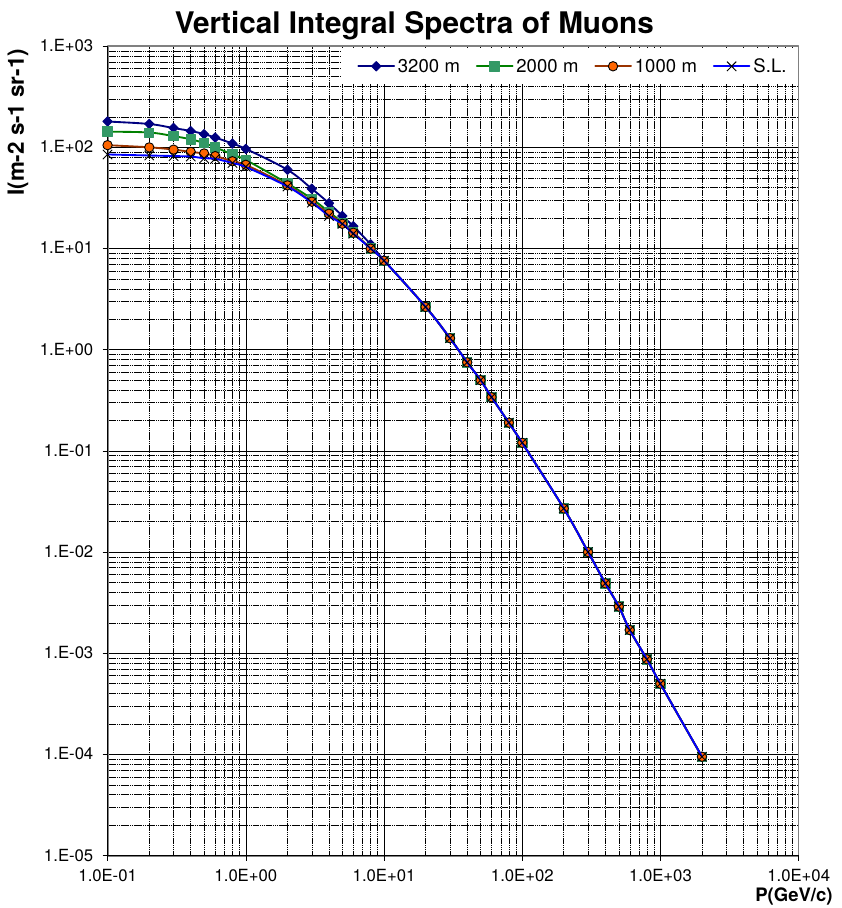
\includegraphics[width=.35\textwidth]{images/dataMuonMom.png} 
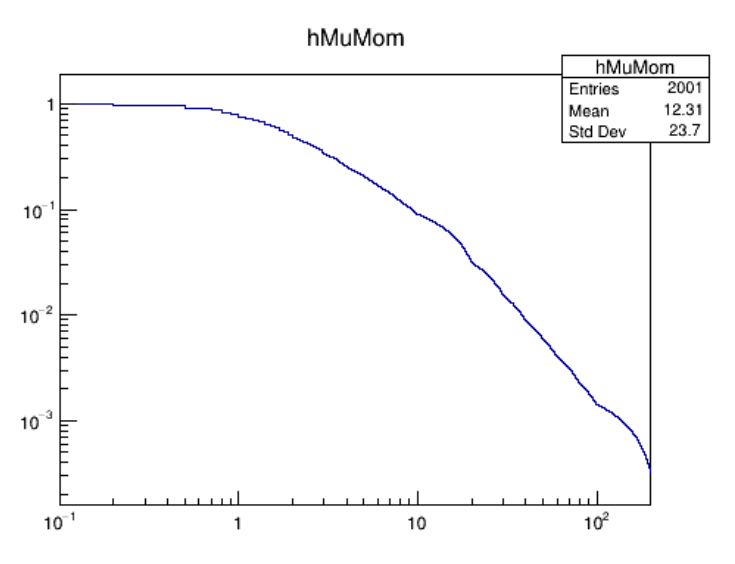
\includegraphics[width=.55\textwidth]{images/hmomfull.png}
\end{figure}
On the right: historgam made from measured integral momentum spectra od muons. Linear interpolation between data points was applied. It is scaled, so the maximum equals 1.
\end{frame}

\begin{frame}{$p_r$ generation}
The algorithm:
\begin{enumerate}
\item a random number $r \in [0, 1)$ is generated (uniform distribution),
\item hMuMom: finding last bin which value is greater than $r$,
\item bin center of the bin (`x value') is the drawn $p_r$ [GeV].
\end{enumerate}
\begin{figure}
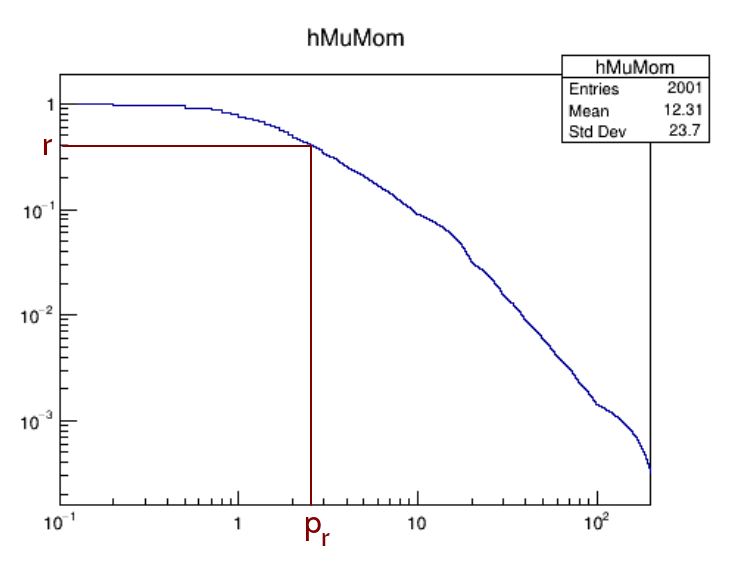
\includegraphics[width=.5\textwidth]{images/drawpr.png} 
\end{figure}
This procedure is very similar to drawing random number using quantile function.
\end{frame}



\begin{frame}{Generation of particles step by step}
\begin{figure}
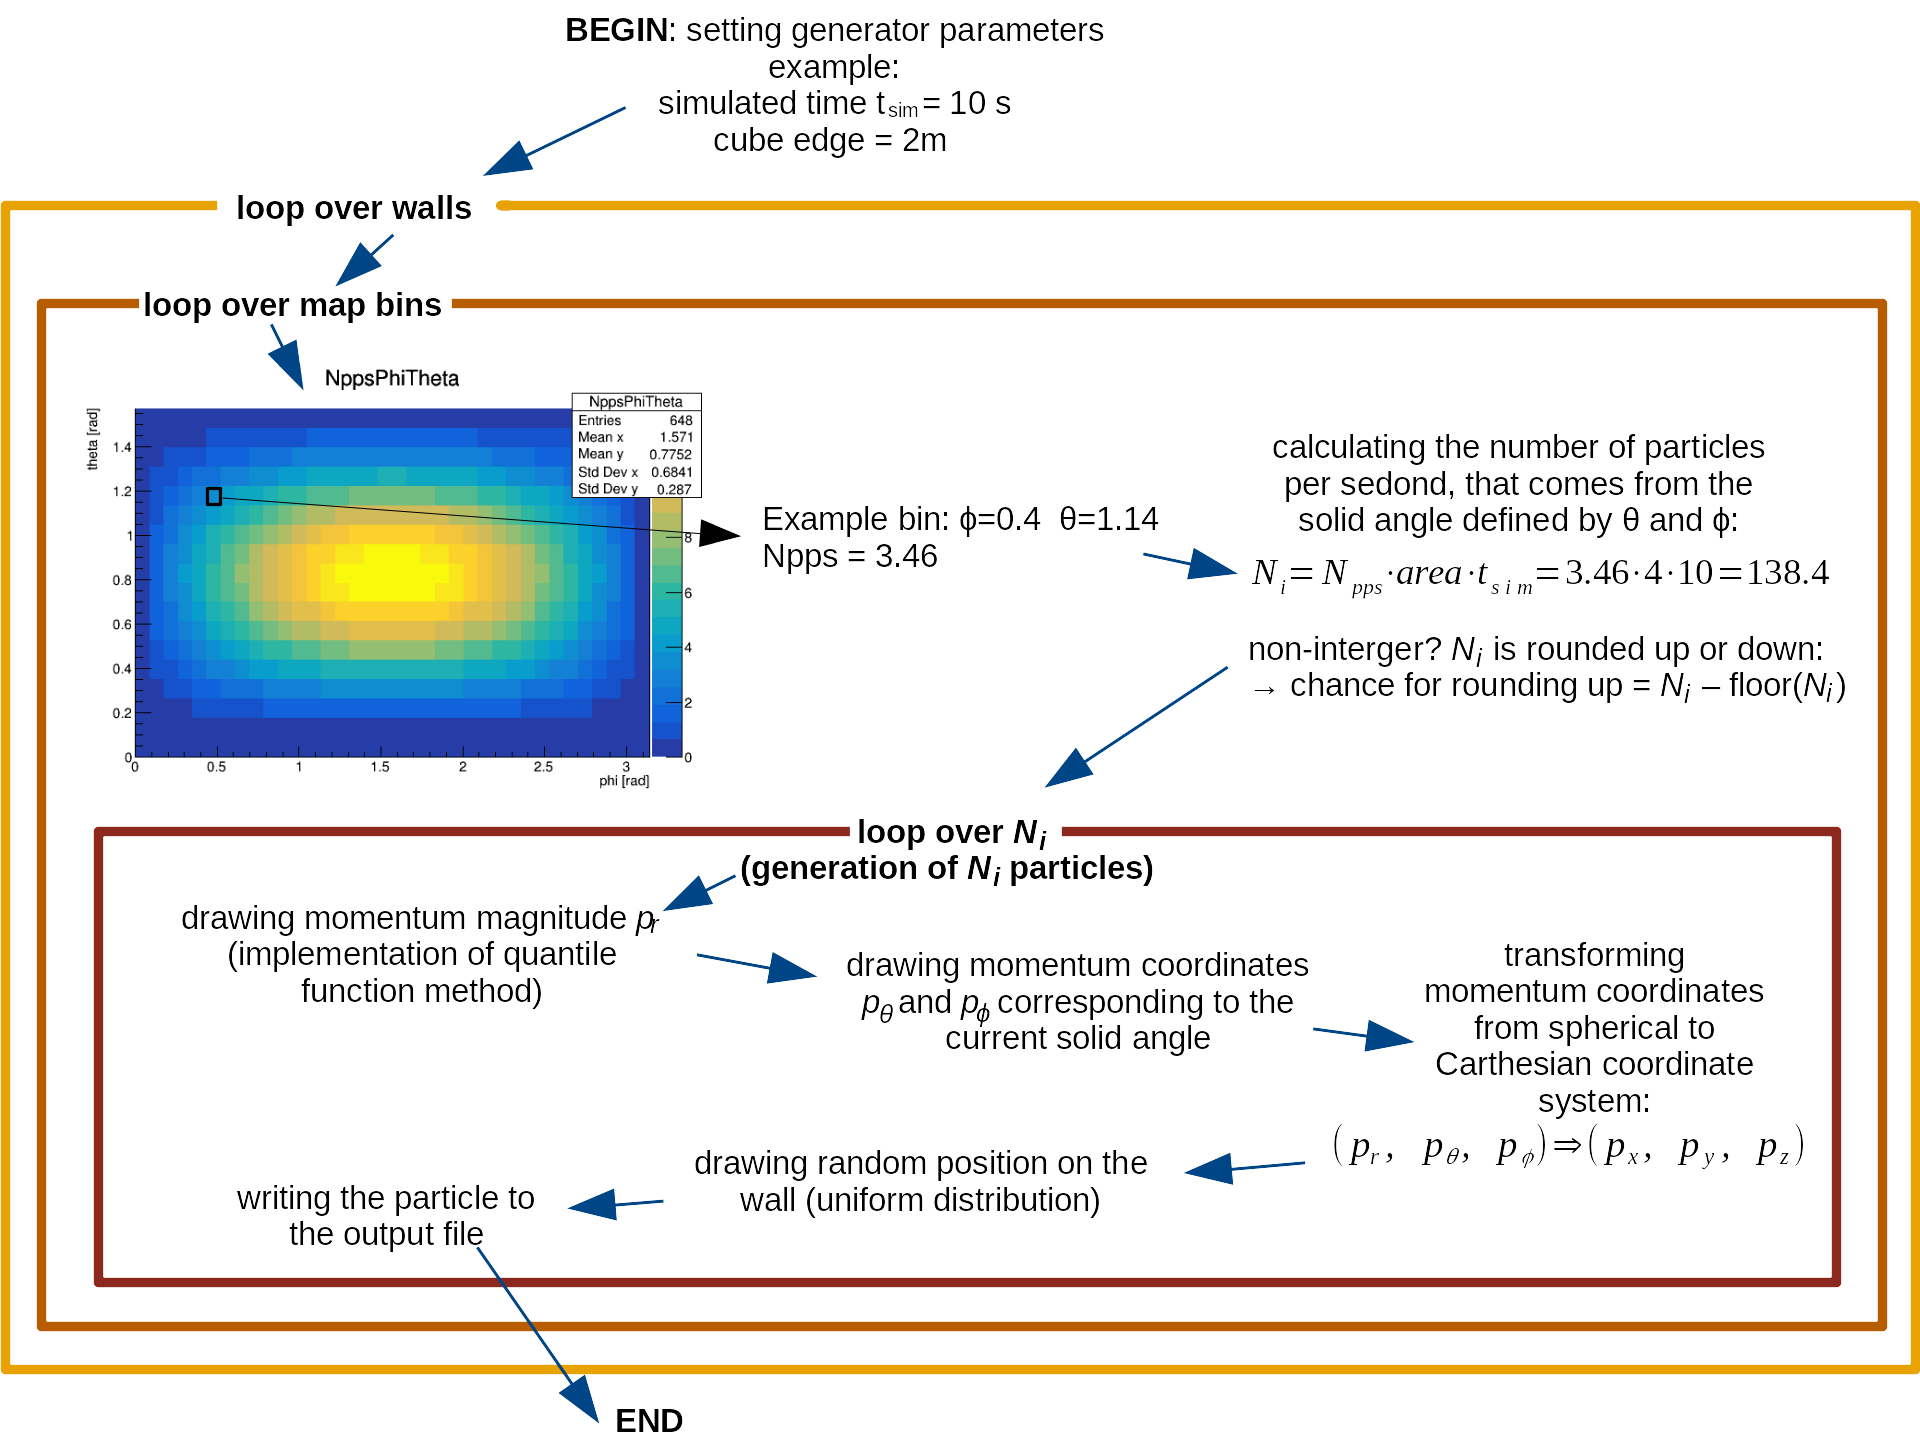
\includegraphics[width=0.87\textwidth]{images/alg.png}
\end{figure}
\end{frame}

\subsection{TrackAnalyzer.cpp}

\begin{frame}{TrackAnalyzer.cpp}
\begin{figure}
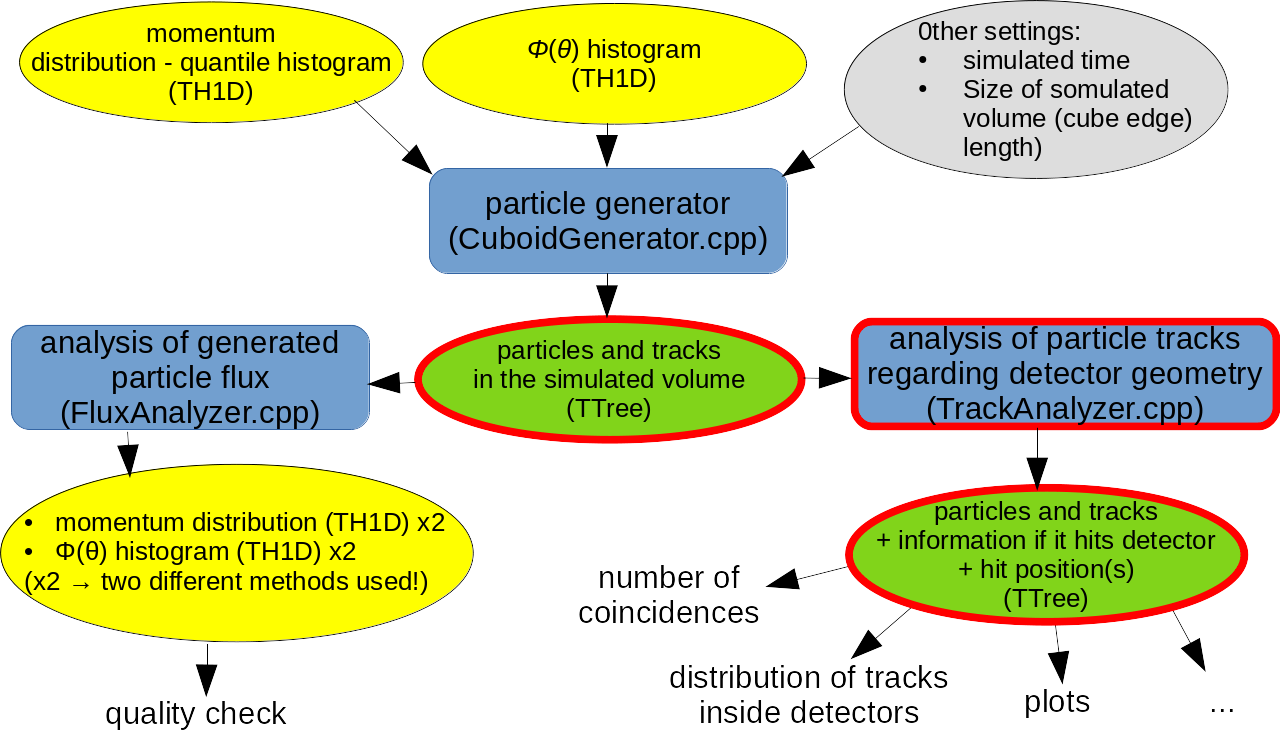
\includegraphics[width=0.9\textwidth]{images/sim_scheme_track.png}%
\end{figure}
\end{frame}

%\begin{frame}[fragile,containsverbatim]{TrackAnalyzer.cpp}
\begin{frame}{TrackAnalyzer.cpp}
Detector elements are defined in the source code (no input config file) -- so far it is good enough for my needs.\\~\\

Implemented shapes (C++ classes):
	\begin{itemize}
	\item Rectangle
	\item Disk
	\item Cylinder
	\end {itemize}
	
Every spahe has a methods that detects if the particle hits the detector module (shape instance) and calculates hit position(s).\\~\\

More detailed description of the classes is presented in the section Technical delails and class description.
\end{frame}


\begin{frame}{TrackAnalyzer.cpp -- input and output tree}
Input tree  from CuboidGenerator -- every entry represents one particle. Variables are stored in different branches:
\begin{figure}
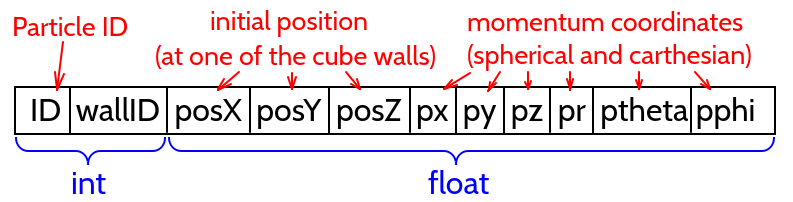
\includegraphics[width=0.5\textwidth]{images/gentree.png}%
\end{figure}

Output tree = inout tree + information if the particle hits each module and hit positions:
\begin{figure}
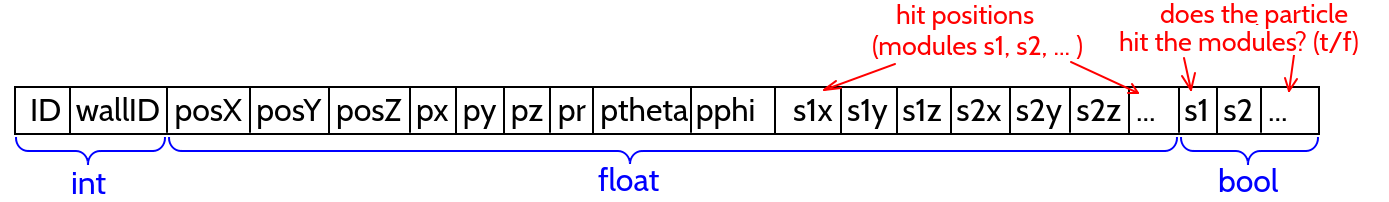
\includegraphics[width=0.9\textwidth]{images/outtree.png}%
\end{figure}

This output tree pattern works fine for simple detector lauoyt, but is not optimal regarding the output file size. For more complicated detector geometries (hundreds of elements), a different way of creating output tree may be needed.
\end{frame}

\begin{frame}{TrackAnalyzer.cpp -- plot of example output}
An example cylinder was defined:
\begin{itemize}
\item radius: r= 1.1 m
\item length L= 3.4 m
\end{itemize}
One can print the points, where the particle track intersects the cylinder surface. Cylinder shape reveals $\Rightarrow$ geometry implementation works correctly
\begin{figure}
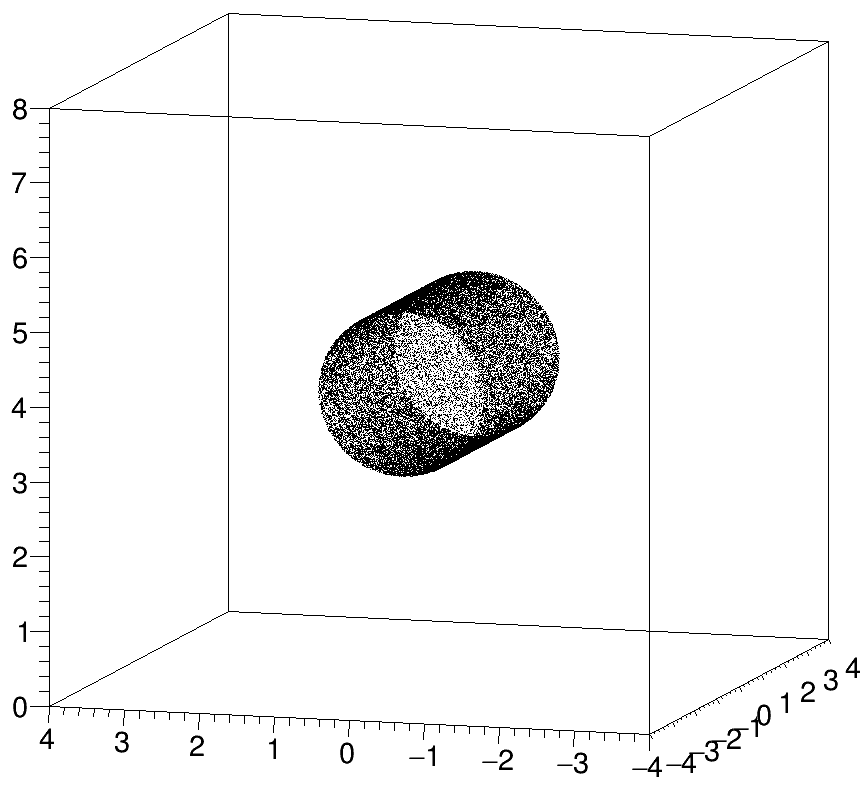
\includegraphics[width=0.45\textwidth]{images/cylinder1.png}%
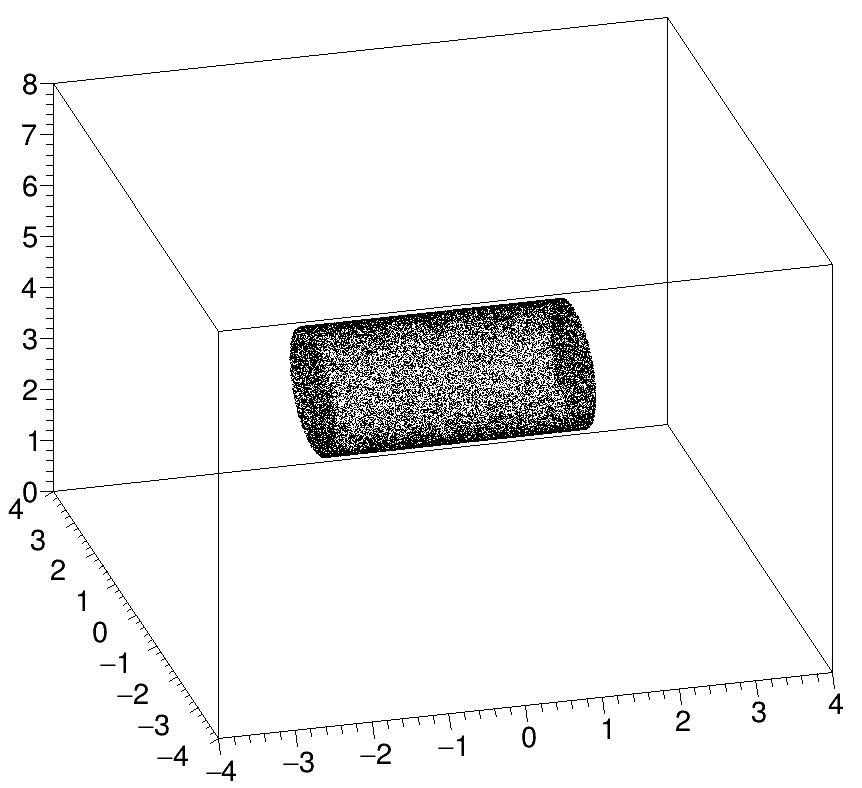
\includegraphics[width=0.45\textwidth]{images/cylinder2.png}%
\end{figure}
\end{frame}

\begin{frame}{TrackAnalyzer.cpp -- plot of example output}
One can also plot a distribution of the path length inside the cylinder:
\begin{figure}
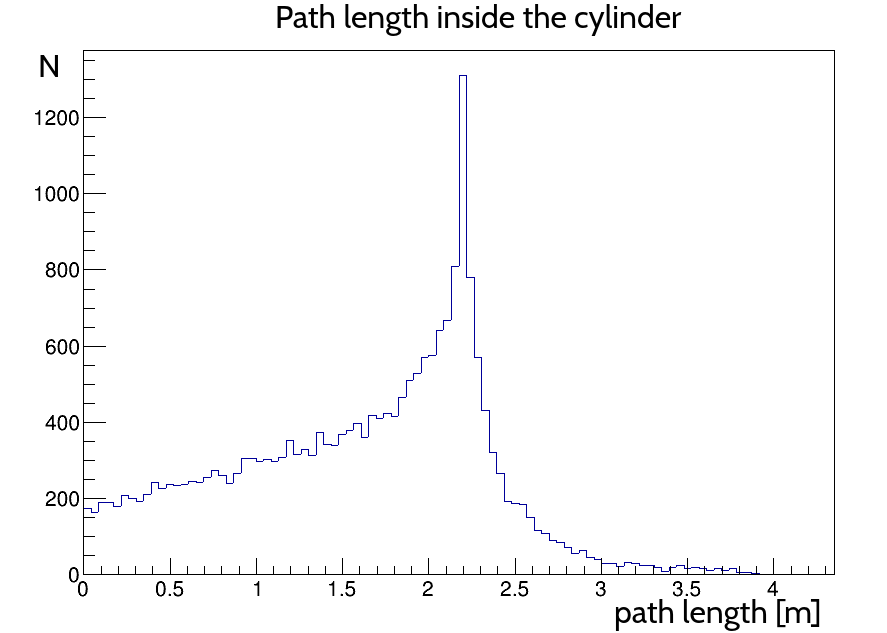
\includegraphics[width=0.58\textwidth]{images/track_dist.png}%
\end{figure}
The distribution is correct:
\begin{itemize}
\item The longest possible path length is $s_{max}=\sqrt{(4r^2 + L^2} \approx 4.1$ [m]
\item Regarding most particles come from the `ceiling', the most common track length should be approximately equal to $2r = 2.2$ [m]
\end{itemize}

\end{frame}

\subsection{FluxAnalyzer.cpp and quality check}

\begin{frame}{FluxAnalyzer.cpp and quality check}
\begin{figure}
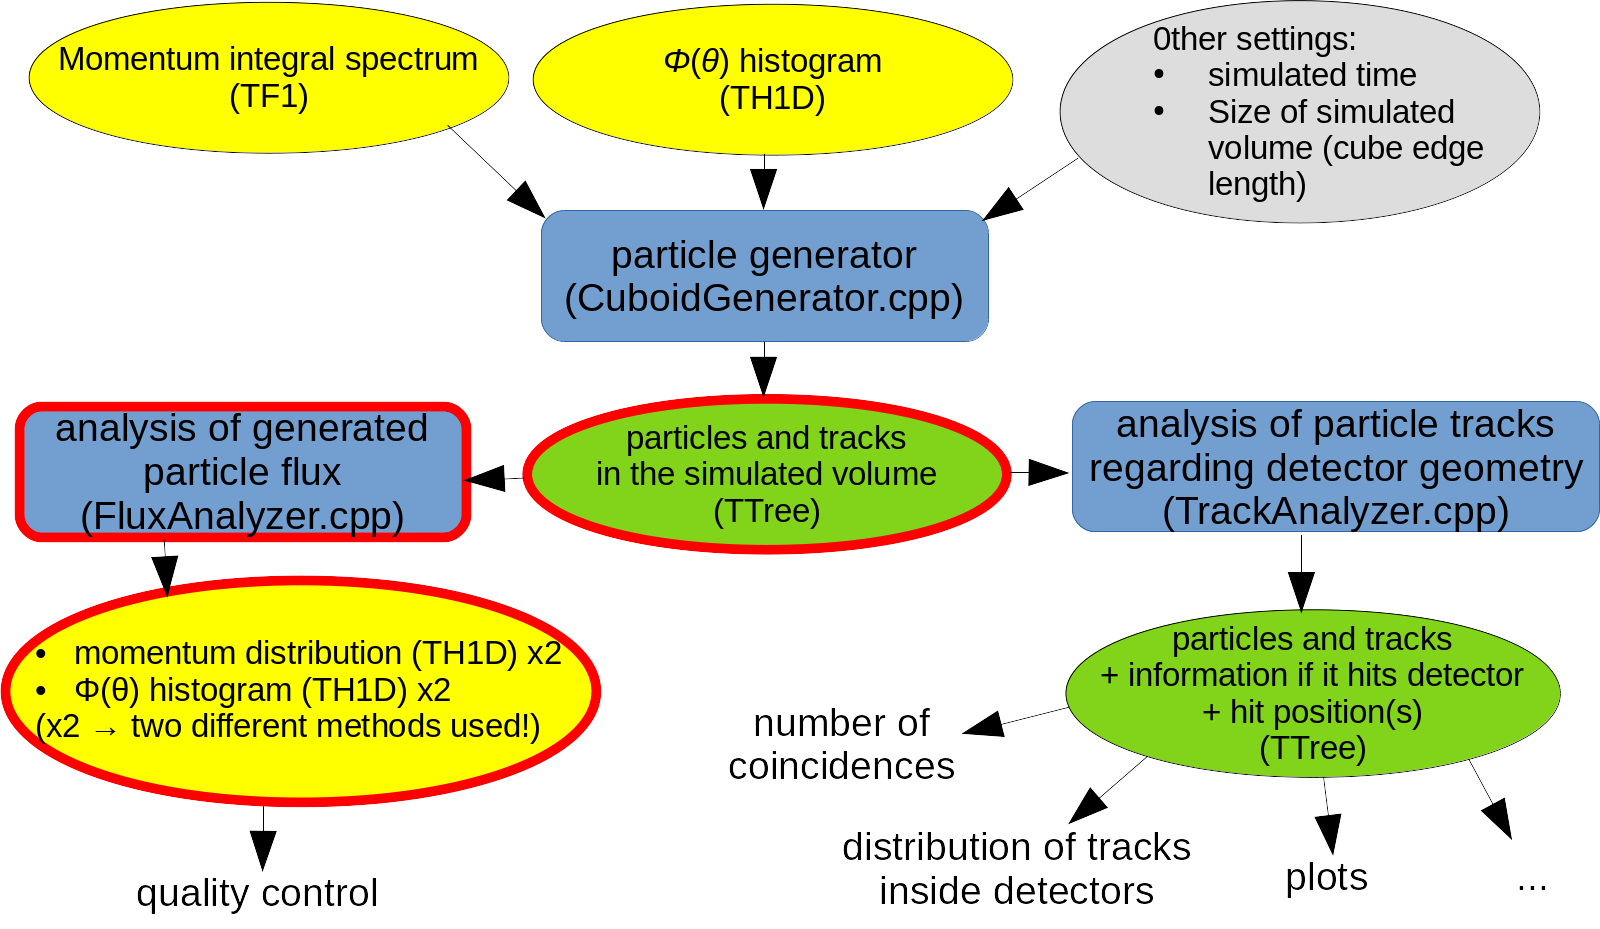
\includegraphics[width=0.9\textwidth]{images/sim_scheme_flux.png}%
\end{figure}
\end{frame}

\begin{frame}{FluxAnalyzer.cpp and quality check}

Quality check of generated particles:
	\begin{itemize}
	\item Are the initial positions ok?
	\item How well $\Phi(\theta)$ and momentum distribution resembles the given experimental data?
	\end {itemize}
\begin{figure}Is it like:\\
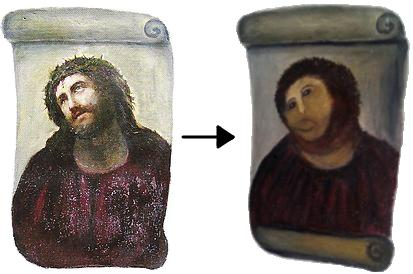
\includegraphics[width=0.29\textwidth]{images/Ecce_Homo.jpg}
\end{figure}
\begin{figure}
or like:\\
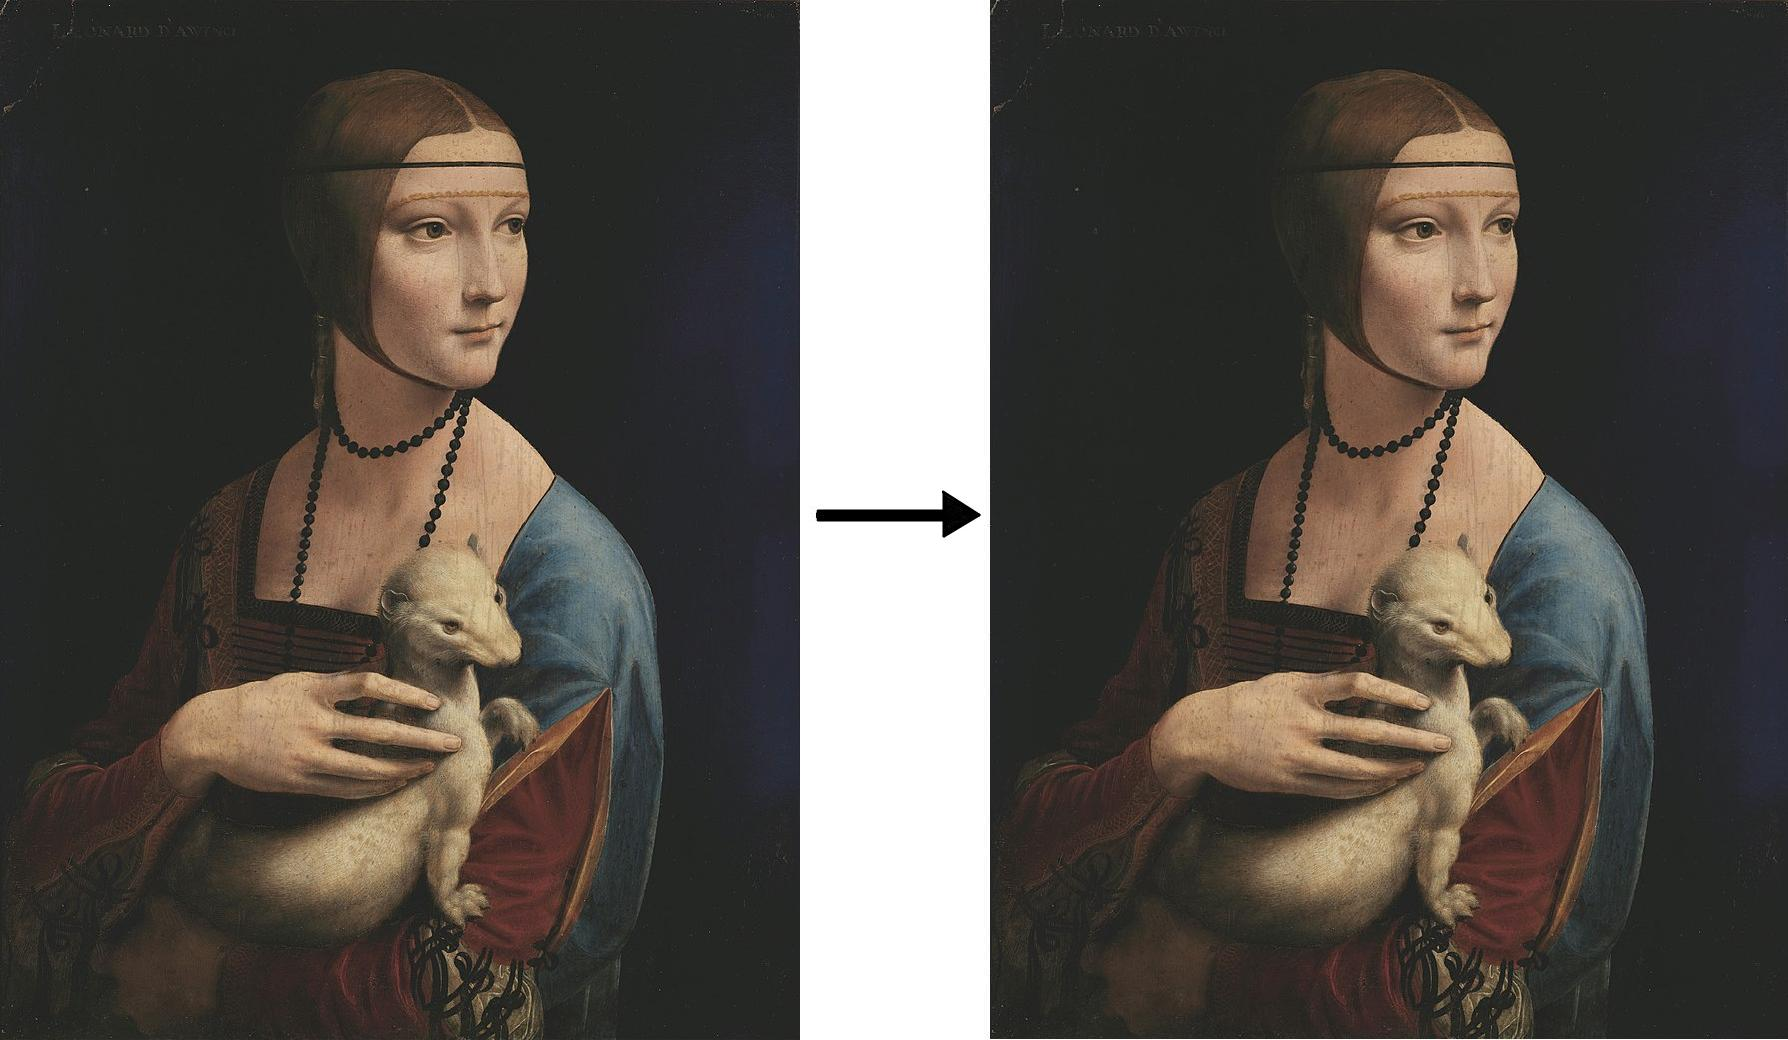
\includegraphics[width=0.28\textwidth]{images/Lady_with_an_Ermine.jpg}\\?
\end{figure}	
\end{frame}

\begin{frame}{FluxAnalyzer.cpp -- two methods of investigating $\Phi(\theta)$}
\begin{enumerate}
\item floor method:
	\begin{enumerate}
	\item Filling $\theta$ distribution histogram with particles that hits the cube floor (bin width: $\Delta \theta$).
	\item Normalizing the distribution to obtain $\Phi(\theta)$. Normalization function:
	\[
	f_n(\theta)=\frac{1}{S \times t_{sim} \times cos(\theta) \times \Omega(\theta)}
	\]
	\end{enumerate}
	
\item rotating rectangle method:
	\begin{enumerate}
	\item Initializing a horizontal rectangle inside the dube the cube. The center of the cube is also the center of this rectangle.
	\item Rotating it through angle $\Delta \theta$. Rotation axis: contains the center of the cube, parallel to the $x$ axis.
	\item filling $\theta$ distribution histogram with particles that hit the rectangle and come from the limited solid angle $\Omega(\theta)$ in front of the rectangle.
	\item Normalizing the distribution to obtain $\Phi(\theta)$. Normalizaing function:
	\[
	f_n(\theta)=\frac{1}{S \times t_{sim} \times \Omega'(\theta)}
	\]
	\end{enumerate}
\end{enumerate}
\end{frame}

\begin{frame}{Quality check: $\theta$ distribution -- floor method}
\begin{figure}
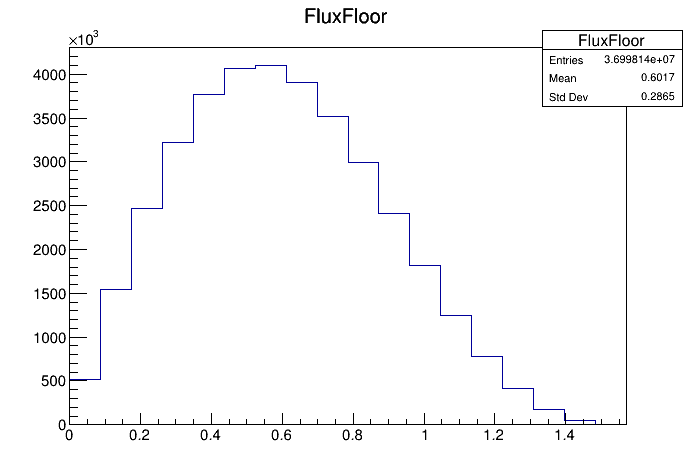
\includegraphics[width=0.42\textwidth]{images/FluxFloor.png}~~
\includegraphics[width=0.42\textwidth]{images/FluxFLoorNormalized.png}\\
Before normalization~~~~~~~~~~~~~~~~~~~~~ Normalized~~~~~\\
~~~~~\includegraphics[width=0.42\textwidth]{images/uFLuxTheta.png}
~~~~~~~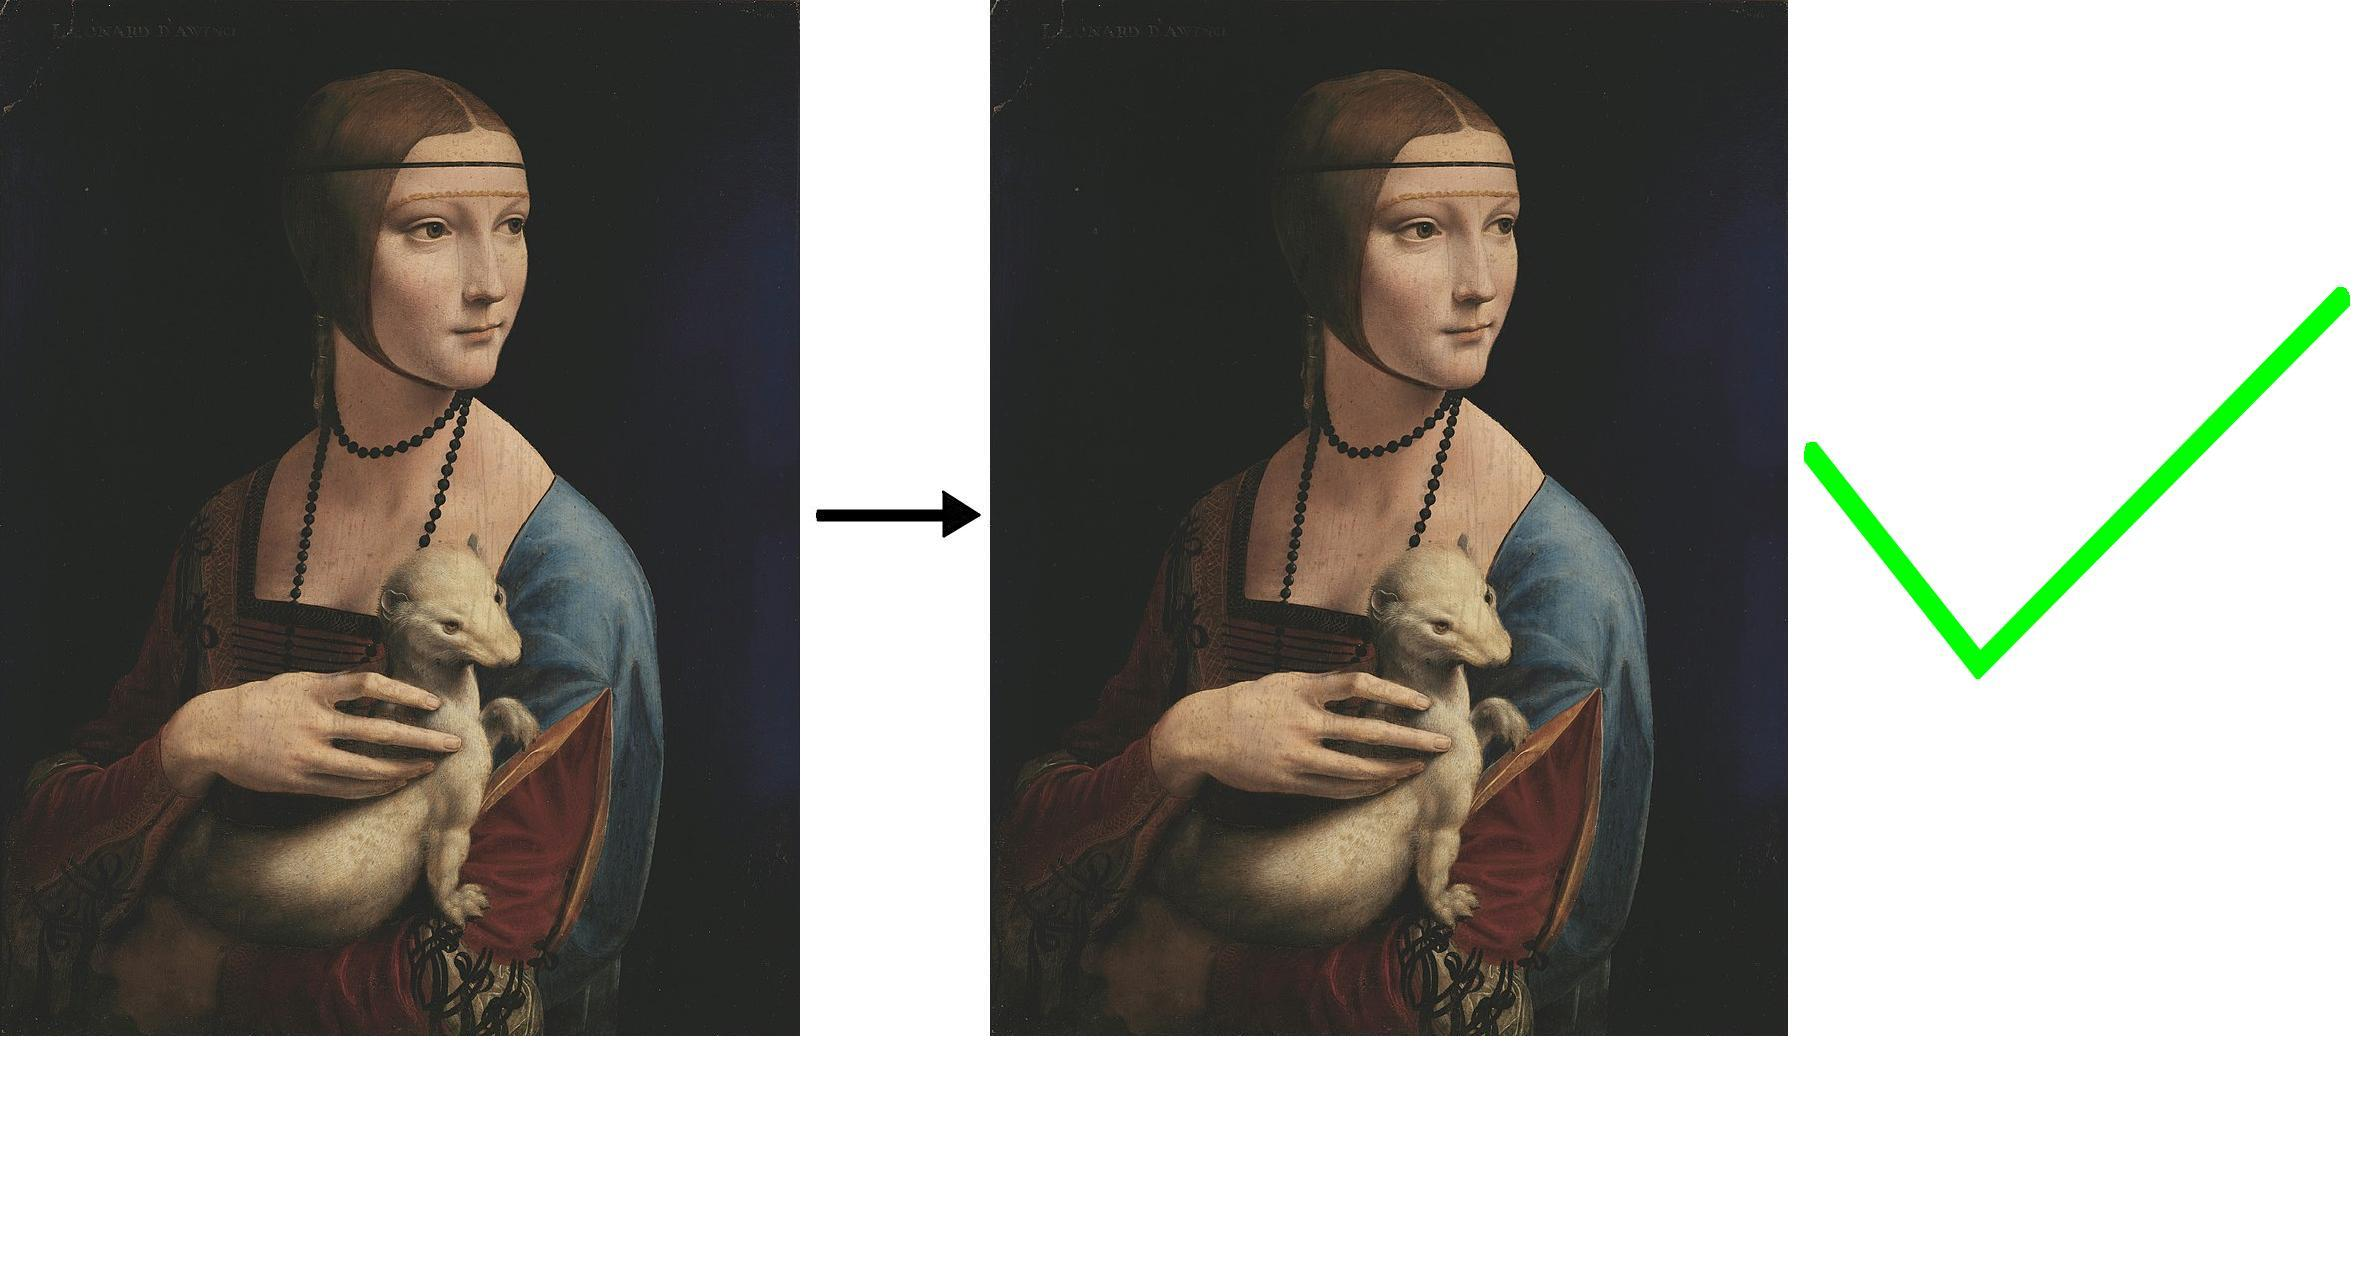
\includegraphics[width=0.42\textwidth]{images/Lady_with_an_Ermine_good.jpg}\\
~Input $\Phi(\theta)$~~~~~~~~~~~~~~~~~~~~~~~~~~~~~Very well!
\end{figure}
\end{frame}

\begin{frame}{Quality check: $\theta$ distribution -- rotating rectangle method}
\begin{figure}
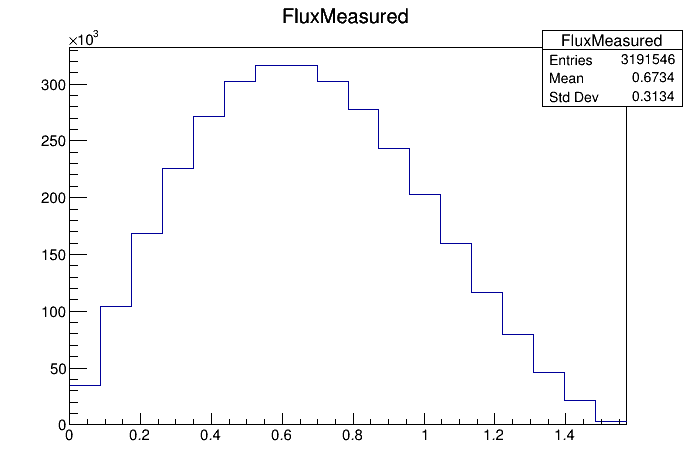
\includegraphics[width=0.42\textwidth]{images/FluxMeasured.png}~~
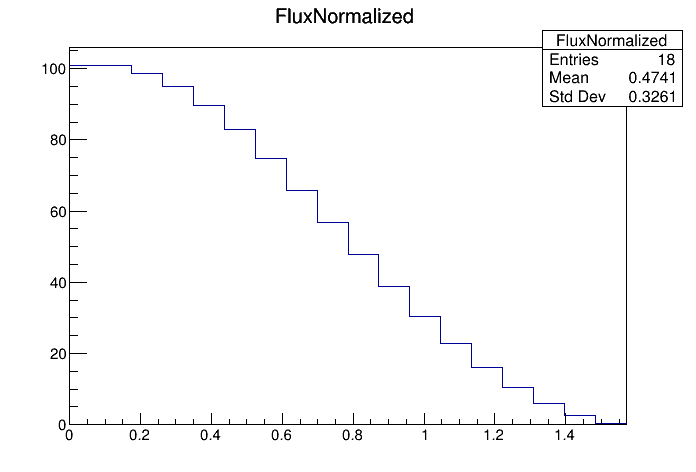
\includegraphics[width=0.42\textwidth]{images/FluxNormalized.png}\\
Before normalization~~~~~~~~~~~~~~~~~~~~~ Normalized~~~~~\\
~~~~~\includegraphics[width=0.42\textwidth]{images/uFLuxTheta.png}
~~~~~~~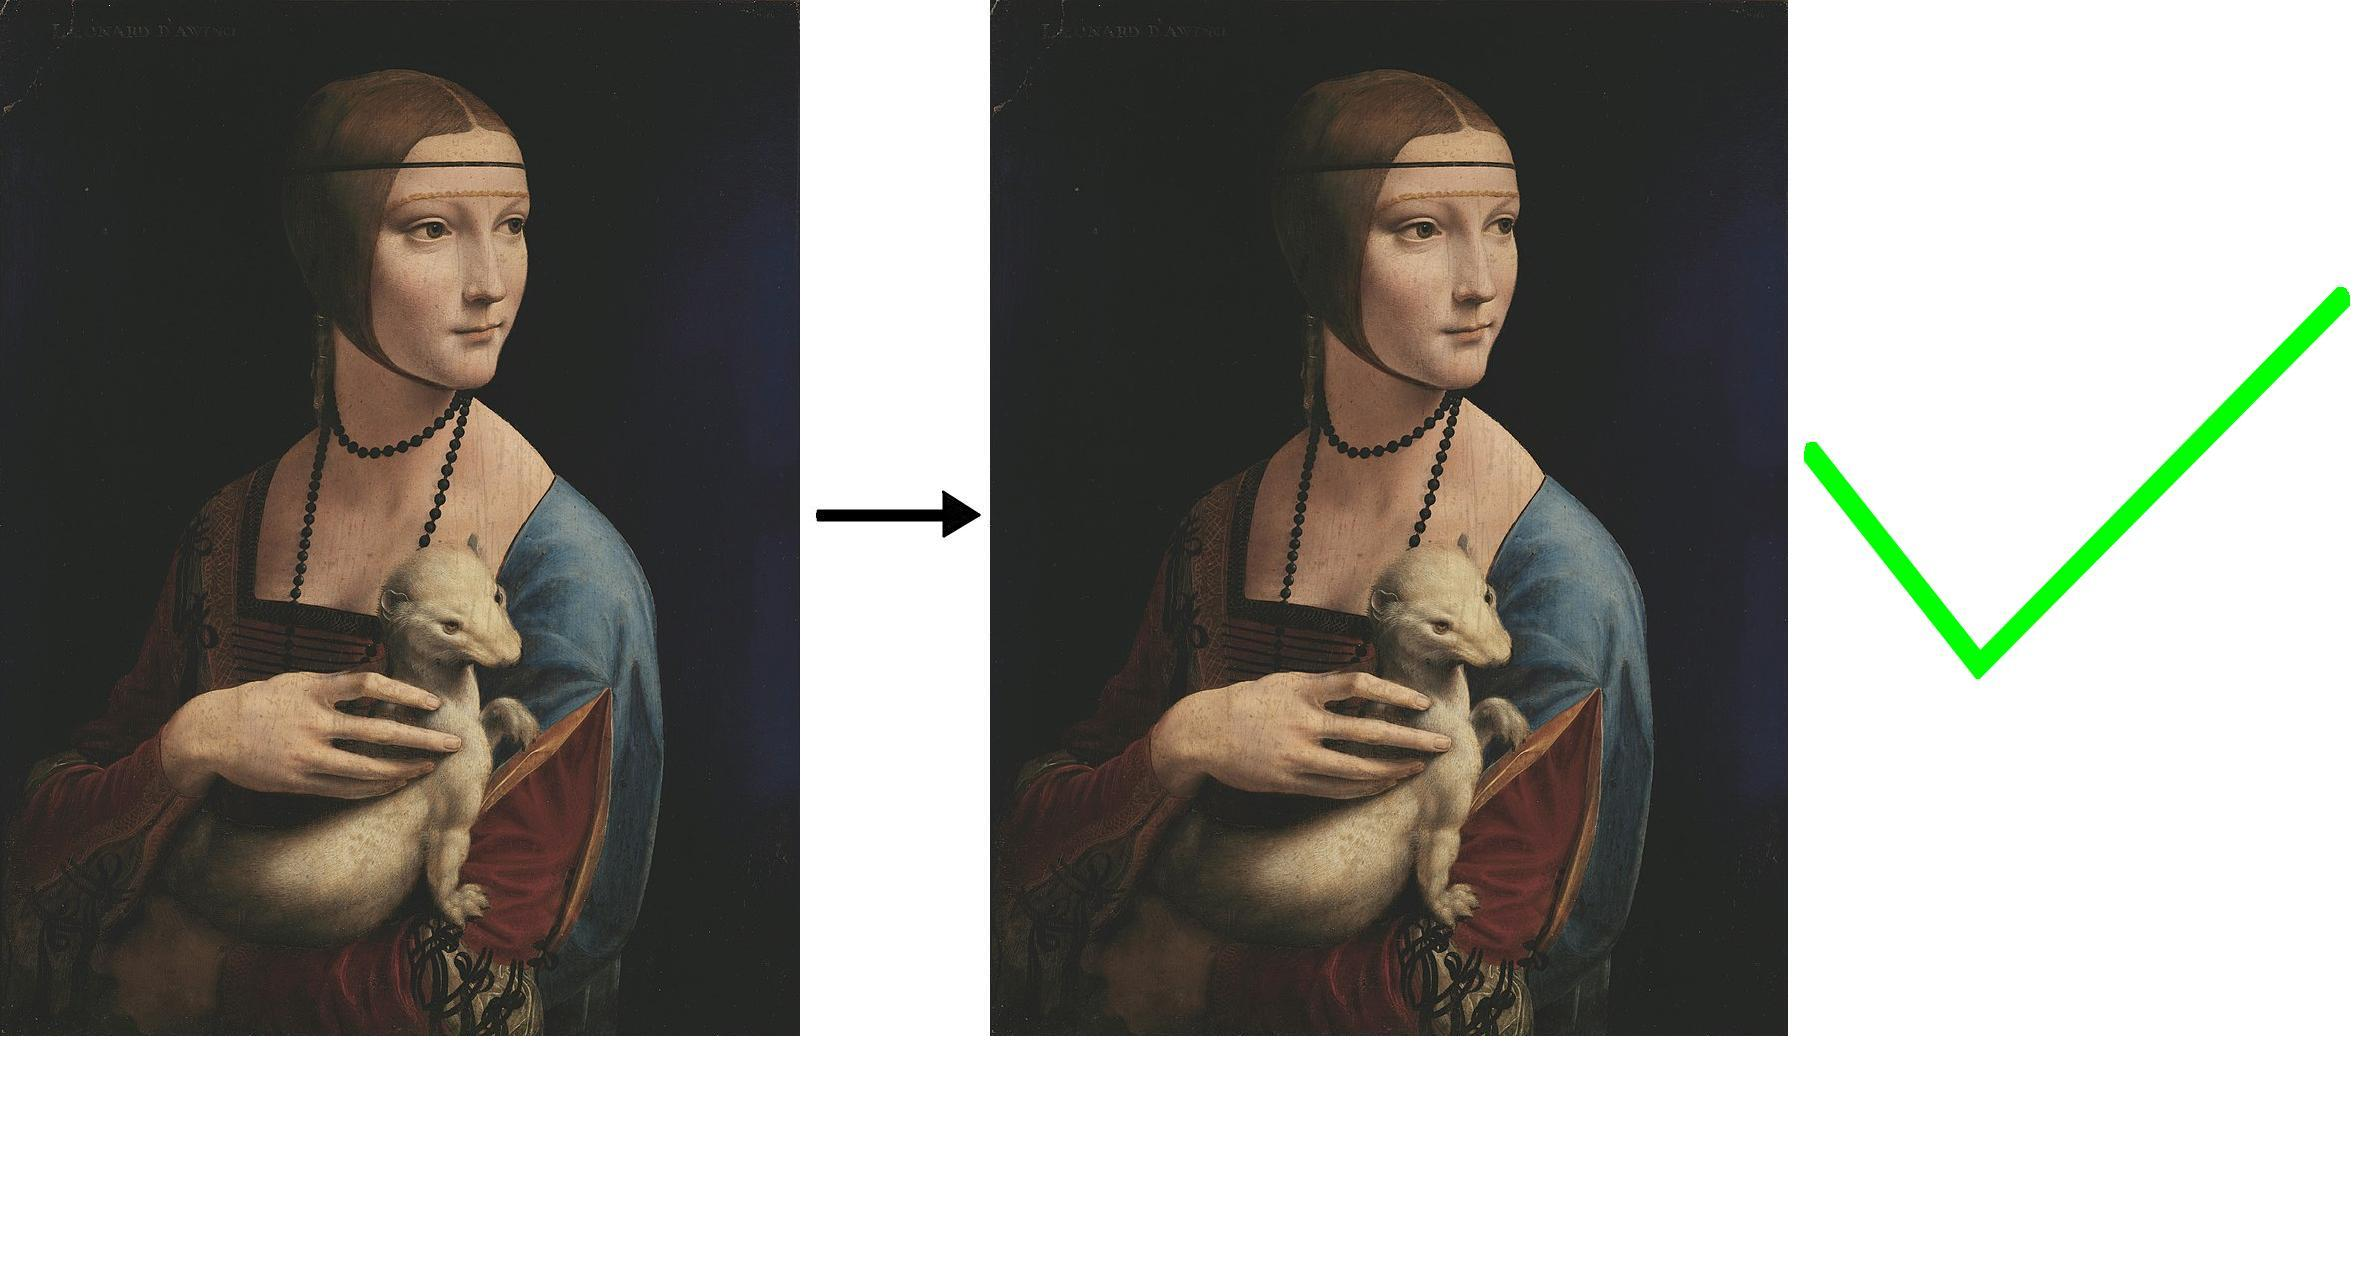
\includegraphics[width=0.42\textwidth]{images/Lady_with_an_Ermine_good.jpg}\\
~~Input $\Phi(\theta)$~~~~~~~~~~~~~~~~~~~~~~~~~~~Even better!
\end{figure}
\end{frame}

\begin{frame}{Quality check: $p_r$}
\begin{figure}
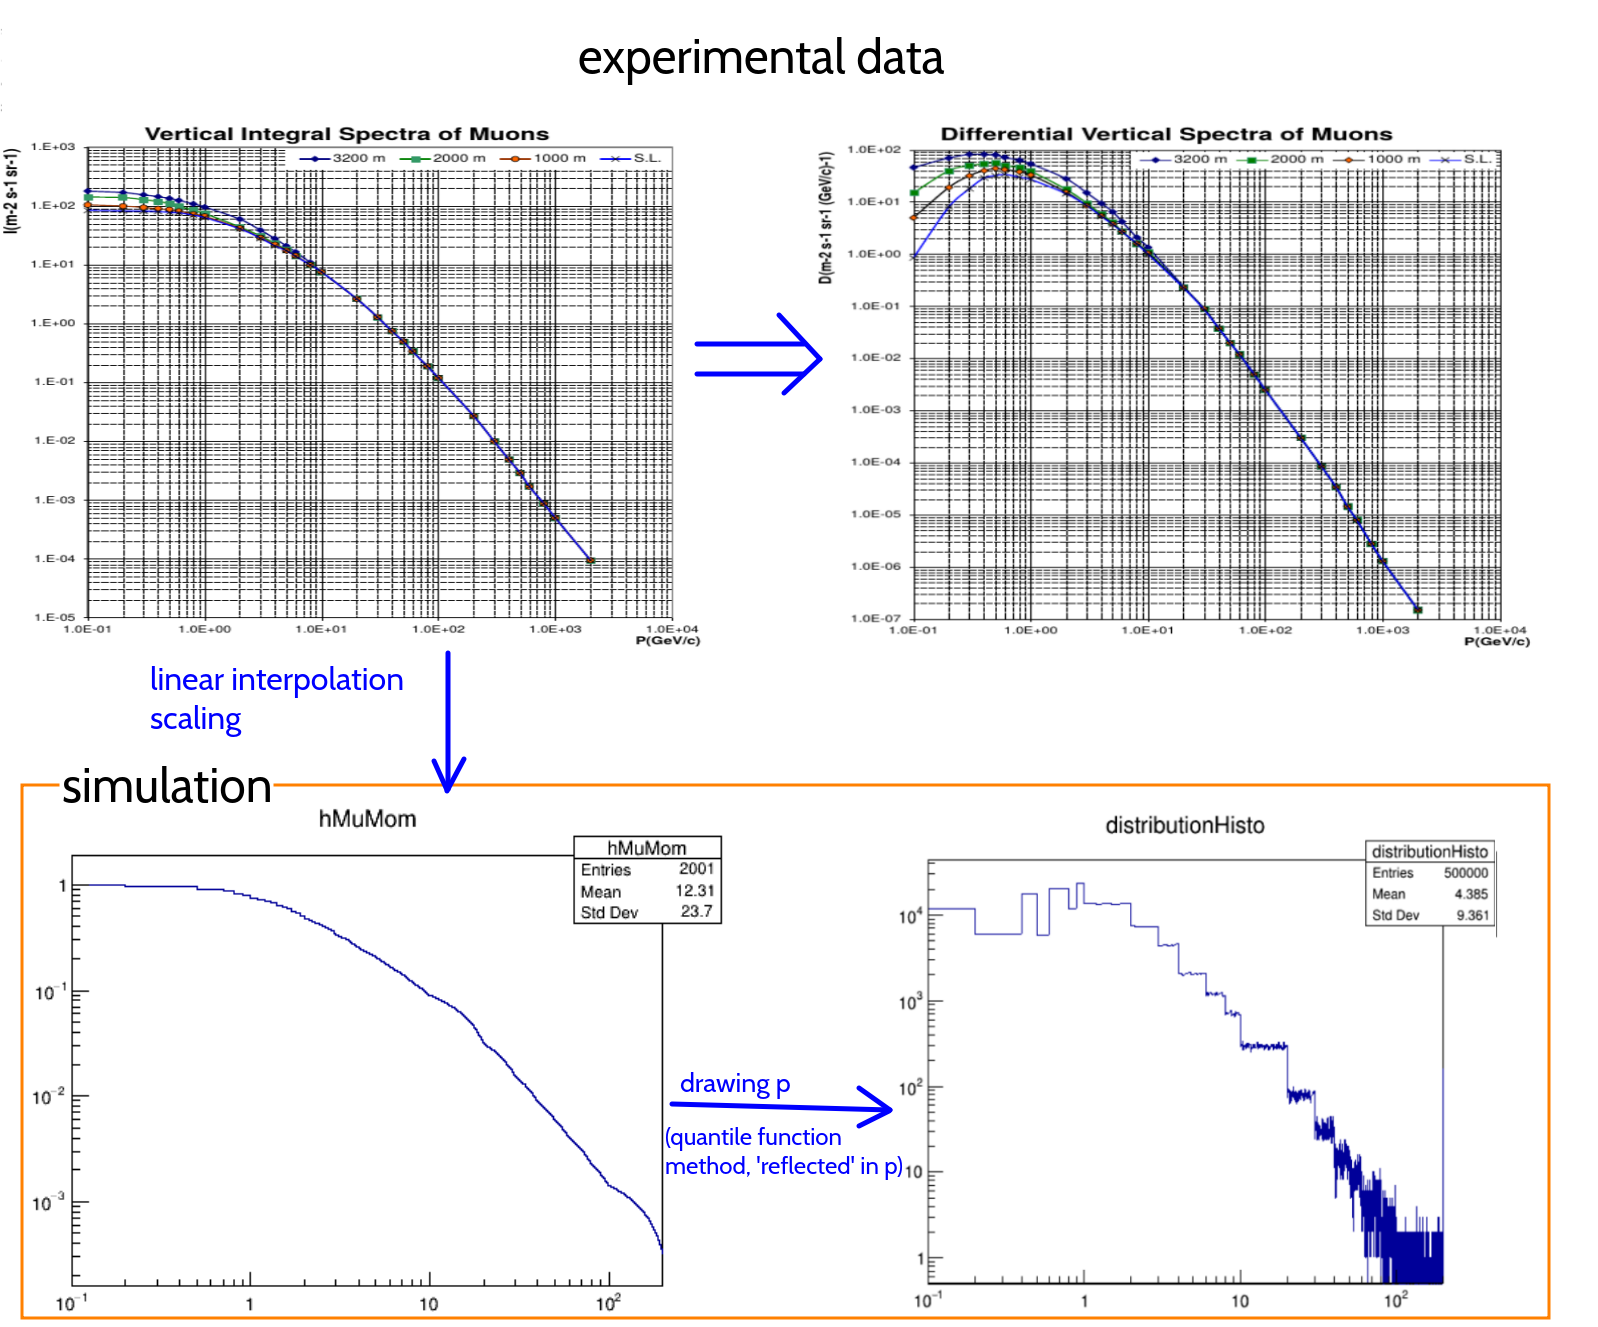
\includegraphics[width=.77\textwidth]{images/pr_distr.png}
\end{figure}
\end{frame}

\begin{frame}{Quality check: $p_r$ evaluation}
Key notes:
\begin{itemize}
\item No normalization implemented for reconstructed $p_r$ $\Rightarrow$ measured and reconstructed $p_r$ cannot be directly compared.
\item The shape of reconstructed $p_r$ seems to be correct, but the reason for size of steps will be investigated.
\end{itemize}

It is yet not obvious whether the $p_r$ reconstruction is as bad as:
\begin{figure}
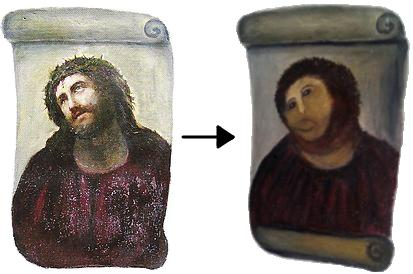
\includegraphics[width=.3\textwidth]{images/Ecce_Homo.jpg}
\end{figure}
and it was good enough to produce some preliminary results, however, the quantile function implementation is planned for improvements.
\end{frame}

\begin{frame}{Quality check: initial positions}
Initial posions are uniformly distributed on each wall of the cube. Also, the highest particle `surface density' of particles is onserved on the cube ceiling. 
\begin{figure}
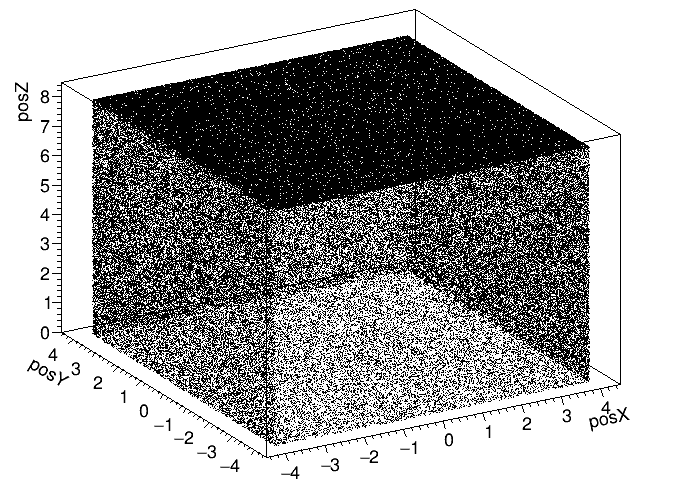
\includegraphics[width=0.70\textwidth]{images/cubefull.png}
\end{figure}
Initial positions are correctly generated!
\end{frame}

\section{Example simulation results}

\begin{frame}
\vfill
\centering
\Huge{Example simulation}

\vfill
\end{frame}

\begin{frame}{Example simulation - general parameters}
General parameters (CuboidGenerator.cpp):
\begin{itemize}
\item cube edge: 8 [m]
\item central point: x=0, y=0, z=4
\item simulated time: 1 [h]
\item simulated $p_{min}=0.1~[\text{GeV/c}]$
\end{itemize}
~\\
For detection, $p_{min} = 1.6~[\text{GeV/c}]$ was assumed. Tracks with lower momenta are ignored (TrackAnalyzer.cpp)
~\\~\\

TPC parameters
\begin{itemize}
\item a single cylinder -- length = 3.4 [m]; radius = 1.1 [m]
\item axis of symmetry: parallel to the X axis, in the center of the cube (y=0, x=4)
\item efficiency $\eta = 1$
\end{itemize}
\end{frame}

\begin{frame}{Simulated detector geometry}
Scintillating modules
\begin{itemize}
\item rectangular modules -- length = 4.784 [m]; width = 0.675 [m] 
\item efficiency $\eta = 0.9$
\item placed around TPC axis
\end{itemize}
\begin{figure}
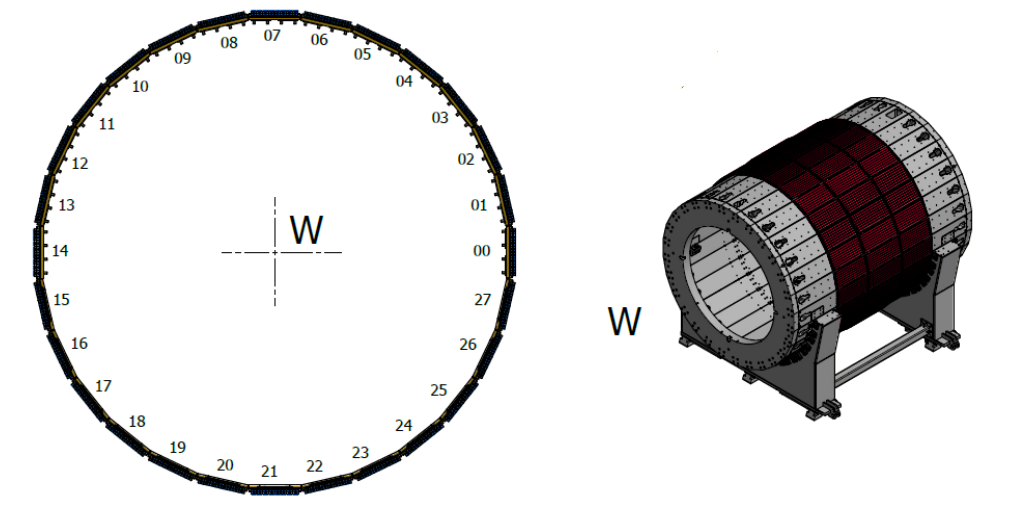
\includegraphics[width=\textwidth]{images/num.png}
\end{figure}
\end{frame}

\begin{frame}{Obtained detector geometry visualisation}
Drawing positions where tracks hits the detectors reveals geometry of the detectors
\begin{figure}
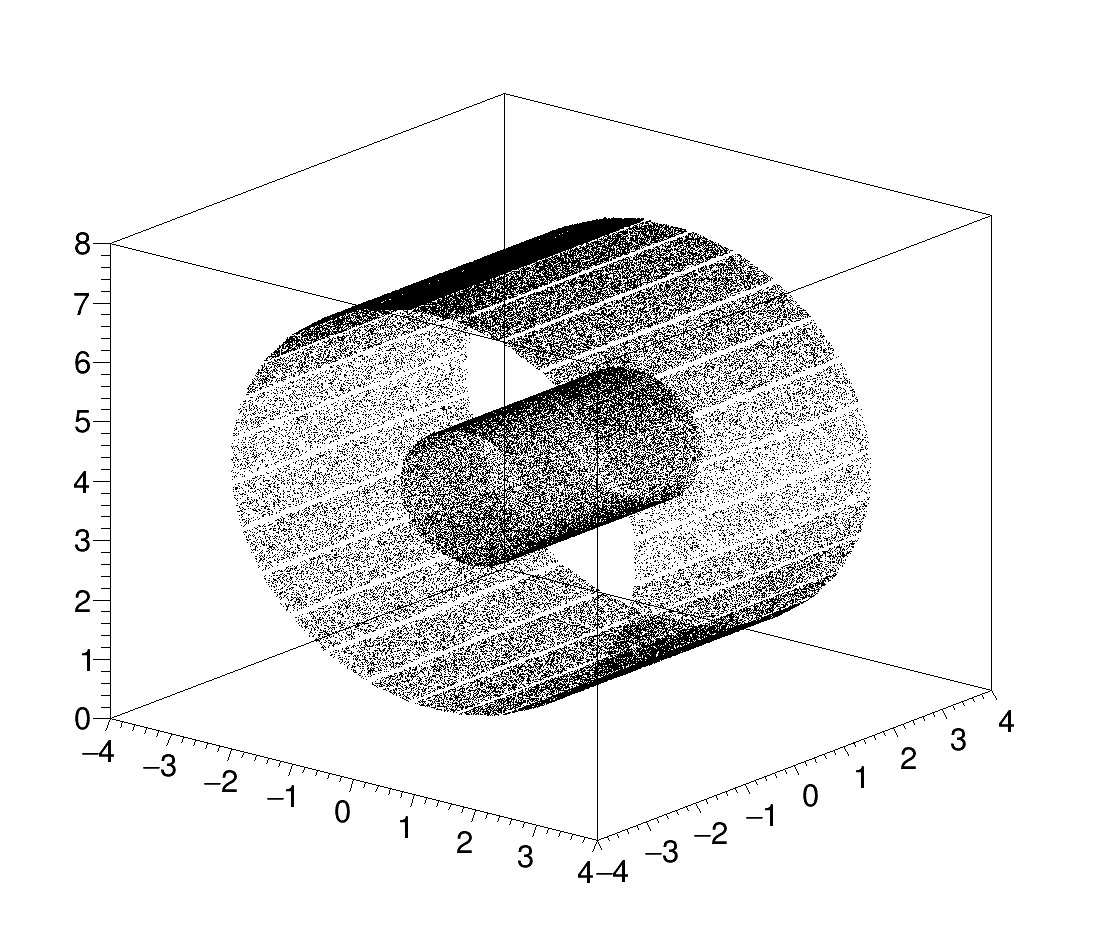
\includegraphics[width=0.65\textwidth]{images/all_modules.png}
\end{figure}
\end{frame}


\begin{frame}{One-to-one coincidences}
\begin{figure}
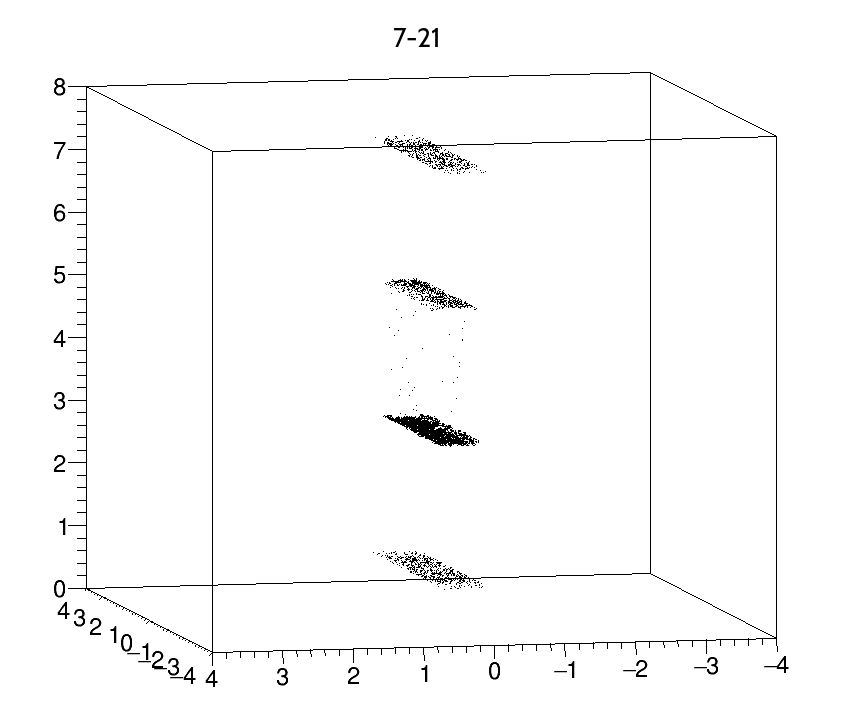
\includegraphics[width=0.7\textwidth]{images/one-to-one.png}
\end{figure}
\end{frame}

\begin{frame}{One-to-one coincidences (with TPC)}
Similar to $cos^2(\theta)$ function -- correct!
\begin{figure}
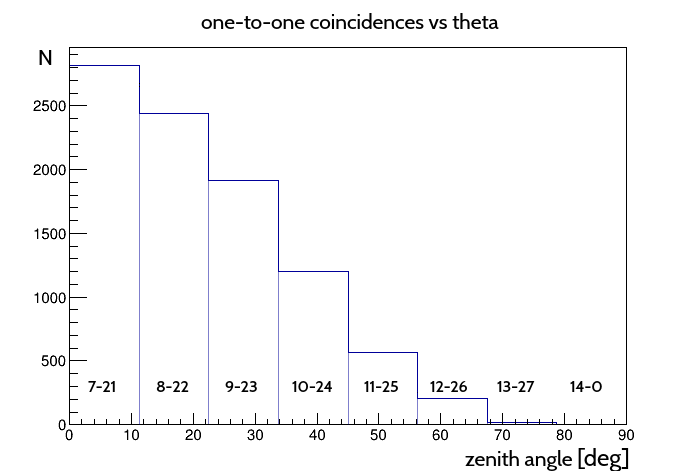
\includegraphics[width=0.65\textwidth]{images/FluxTheta.png}
\includegraphics[width=0.34\textwidth]{images/nocoin.png}
\end{figure}
\end{frame}

\begin{frame}{Layout 1: modules close to each other}
\begin{figure}
\includegraphics[width=0.65\textwidth]{images/close.png}
\end{figure}
\end{frame}

\begin{frame}{Layout 1: modules close to each other}
\begin{itemize}
\item (6 or 7 or 8) and (20 or 21 or 22) and TPC -- 23341 coincidences per hour
\item (9 or 10 or 11) and (23 or 24 or 25) and TPC -- 15415 coincidences per hour
\item (12 or 13 or 14) and (26 or 27 or 0) and TPC -- 1956 coincidences per hour
\begin{figure}
\includegraphics[width=0.4\textwidth]{images/nocoin.png}
\end{figure}
\end{itemize}
\end{frame}

\begin{frame}{Layout 2: space between modules}
\begin{figure}
\includegraphics[width=0.65\textwidth]{images/spaces.png}
\end{figure}
\end{frame}

\begin{frame}{Layout 2: space between modules}
\begin{itemize}
\item (5 or 7 or 9) and (19 or 21 or 23) and TPC -- 31402 coincidences per hour
\item (10 or 12 or 14) and (24 or 26 or 0) and TPC -- 4892 coincidences per hour
\begin{figure}
\includegraphics[width=0.4\textwidth]{images/nocoin.png}
\end{figure}
\end{itemize}
\end{frame}

\section{Code description}

\begin{frame}
\vfill
\centering
\Huge{Code description}

\vfill
\end{frame}

\subsection{Project class structure}
\subsection{Description of selected classes}
\subsection{License}

\begin{frame}
\vfill
\centering
\Huge{Thank ypu for your attention!}

\vfill
\end{frame}

%backup
%%%%%%%%%%%%%%%%%%%%%%%%%%%%%%%%%%%%%%%%%%%%
%\appendix
%\backupbegin
%\begin{frame}{Mapping $\Phi(\theta, \phi)$ for each wall}
%For all walls reconstruction works fine
%\begin{figure}
%\includegraphics[width=0.49\textwidth]{images/Wall1FluxMap.png}
%\includegraphics[width=0.49\textwidth]{images/wall1Map.png}
%\caption{TH2D $\Phi(\theta, \phi)$ map for the cube ceiling: generated (left), reconstructed (right).}
%\end{figure}
%\end{frame}
%\backupend
\end{document}